\documentclass[table]{beamer}
%[]中可以使用draft、handout、screen、transparency、trancompress、compress等参数

%指定beamer的模式与主题
\mode<presentation>
{
  \usetheme{Madrid}
%\usetheme{Boadilla}
%\usecolortheme{default}
%\usecolortheme{orchid}
%\usecolortheme{whale}
%\usefonttheme{professionalfonts}
}

%\usetheme{Madrid}
%这里还可以选择别的主题:Bergen, Boadilla, Madrid, AnnArbor, CambridgeUS, Pittsburgh, Rochester, Warsaw, ...
%有导航栏的Antibes, JuanLesPins, Montpellier, ...
%有内容的Berkeley, PaloAlto, Goettingen, Marburg, Hannover, ...
%有最小导航栏的Berlin, Ilmenau, Dresden, Darmstadt, Frankfurt, Singapore, Szeged, ...
%有章和节表单的Copenhagen, Luebeck, Malmoe, Warsaw, ...

%\usecolortheme{default}
%设置内部颜色主题(这些主题一般改变block里的颜色);这个主题一般选择动物来命名
%这里还可以选择别的颜色主题,如默认的和有特别目的的颜色主题default,structure,sidebartab,全颜色主题albatross,beetle,crane,dove,fly,seagull,wolverine,beaver

%\usecolortheme{orchid}
%设置外部颜色主题(这些主题一般改变title里的颜色);这个主题一般选择植物来命名
%这里还可以选择别的颜色主题,如默认的和有特别目的的颜色主题lily,orchid,rose

%\usecolortheme{whale}
%设置字体主题;这个主题一般选择海洋动物来命名
%这里还可以选择别的颜色主题,如默认的和有特别目的的颜色主题whale,seahorse,dolphin

%\usefonttheme{professionalfonts}
%类似的还可以定义structurebold,structuresmallcapsserif,professionalfonts

% 控制 beamer 的风格,可以根据自己的爱好修改
%\usepackage{beamerthemesplit} %使用 split 风格
%\usepackage{beamerthemeshadow} %使用 shadow 风格
%\usepackage[width=2cm,dark,tab]{beamerthemesidebar}

%插入音标
%\usepackage{tipa}
%\AtBeginDocument{
  %\renewcommand\textipa{\fontencoding{T3}\selectfont}
%}
%\AtBeginDocument{
  %\renewcommand\textipa[2][r]{{\fontfamily{cm#1}\tipaencoding #2}}
%}
%\renewenvironment{IPA}[1][r]
 %{\fontfamily{cm#1}\tipaencoding}
 %{}

% 设定英文字体
%\usepackage{fontspec}
% Fix bugs for fontspec in TeXLive2015
\ifdefined\suppressfontnotfounderror
  \expandafter\let\csname xetex_suppressfontnotfounderror:D\endcsname
    \suppressfontnotfounderror
\else
  \expandafter\let\csname xetex_suppressfontnotfounderror:D\endcsname
    \luatexsuppressfontnotfounderror
\fi
\usepackage[no-math]{fontspec}
\setmainfont{Times New Roman}
\setsansfont{Arial}
\setmonofont{Courier New}

% 设定中文字体
\usepackage[BoldFont,SlantFont,CJKchecksingle,CJKnumber]{xeCJK}
%\setCJKmainfont[BoldFont={Adobe Heiti Std},ItalicFont={Adobe Kaiti Std}]{Adobe Song Std}
\setCJKmainfont[BoldFont={Adobe Heiti Std},ItalicFont={Adobe Kaiti Std}]{WenQuanYi Micro Hei}
\setCJKsansfont{Adobe Heiti Std}
\setCJKmonofont{Adobe Fangsong Std}
\punctstyle{hangmobanjiao}

\defaultfontfeatures{Mapping=tex-text}
\usepackage{xunicode}
\usepackage{xltxtra}

\XeTeXlinebreaklocale "zh"
\XeTeXlinebreakskip = 0pt plus 1pt minus 0.1pt

\usepackage{setspace}
\usepackage{colortbl,xcolor}
\usepackage{hyperref}
%\hypersetup{xetex,bookmarksnumbered=true,bookmarksopen=true,pdfborder=1,breaklinks,colorlinks,linkcolor=blue,filecolor=black,urlcolor=cyan,citecolor=green}
\hypersetup{xetex,bookmarksnumbered=true,bookmarksopen=true,pdfborder=1,breaklinks,colorlinks,linkcolor=cyan,filecolor=black,urlcolor=blue,citecolor=green}

% 插入图片
\usepackage{graphicx}
\graphicspath{{figures/}}
% 图文混排
%\usepackage{picins}
\usepackage{floatflt}

% 可能用到的包
\usepackage{amsmath,amssymb}
%插入多媒体
%\usepackage{media9}
%\usepackage{movie15}
\usepackage{multimedia}
\usepackage{multicol}
\usepackage{multirow}

% 定义一些自选的模板,包括背景、图标、导航条和页脚等,修改要慎重
% 设置背景渐变由10%的红变成10%的结构颜色
%\beamertemplateshadingbackground{red!10}{structure!10}
%\beamertemplatesolidbackgroundcolor{white!90!blue}
% 使所有隐藏的文本完全透明、动态,而且动态的范围很小
\beamertemplatetransparentcovereddynamic
% 使itemize环境中变成小球,这是一种视觉效果
\beamertemplateballitem
% 为所有已编号的部分设置一个章节目录,并且编号显示成小球
\beamertemplatenumberedballsectiontoc
% 将每一页的要素的要素名设成加粗字体
\beamertemplateboldpartpage

% item逐步显示时,使已经出现的item、正在显示的item、将要出现的item呈现不同颜色
\def\hilite<#1>{
 \temporal<#1>{\color{gray}}{\color{blue}}
    {\color{blue!25}}
}

\renewcommand{\today}{\number\year 年 \number\month 月 \number\day 日}

%五角星
\usepackage{MnSymbol}

%去除图表标题中的figure等
\usepackage{caption}
\captionsetup{labelformat=empty,labelsep=none}

\usepackage{tabu}
\usepackage{multirow}
%表格自动换行
\usepackage{tabularx} 

% 千分号
%\usepackage{textcomp}

%罗马数字
\makeatletter
\newcommand{\rmnum}[1]{\romannumeral #1}
\newcommand{\Rmnum}[1]{\expandafter\@slowromancap\romannumeral #1@}
\makeatother

%分栏
\usepackage{multicol}

%\usepackage{enumitem}
%\usepackage{enumerate}

%键盘
\usepackage{keystroke}

%心形
%\usepackage{fdsymbol}

%插入源代码
\usepackage{listings}
\lstset{
  language=perl,                  % 程序语言名称:TeX, Perl, R, sh, bash, Awk
  basicstyle=\normalsize\tt,      %\tt指monospace字体族,程序源代码使用此族字体表示更加美观
  numbers=left,                   % 行号位置(左侧)
  numberstyle=\small,             % 行号字体的字号
  stepnumber=1,                   % 行号的显示步长
  numbersep=5pt,                  % 行号与代码间距
  backgroundcolor=\color{white},  % 背景色;需要 \usepackage{color}
  showspaces=false,               % 不显示空格
  showstringspaces=false,         % 不显示代码字符串中的空格标记
  showtabs=false,                 % 不显示 TAB
  tabsize=4, 
  frame=shadowbox,                % 把代码用带有阴影的框圈起来
  captionpos=b,                   % 标题位置
  breaklines=true,                % 对过长的代码自动断行
  breakatwhitespace=false,        % 断行只在空格处
  extendedchars=false,            % 解决代码跨页时,章节标题,页眉等汉字不显示的问题
  %escapeinside={\%*}{*},         % 跳脱字符,添加注释,暂时离开 listings 
  %escapeinside=``,
  commentstyle=\color{red!50!green!50!blue!50}\tt,  %浅灰色的注释
  rulesepcolor=\color{red!20!green!20!blue!20},     %代码块边框为淡青色
  keywordstyle=\color{blue!70}\bfseries\tt,         %代码关键字的颜色为蓝色,粗体
  identifierstyle=\tt,
  stringstyle=\tt,                % 代码字符串的特殊格式
  keepspaces=true,
  breakindent=1em,
  %breakindent=22pt,
  %breakindent=4em,
  breakautoindent=true,
  flexiblecolumns=true,
  aboveskip=1em,                  %代码块边框
  xleftmargin=2em,
  xrightmargin=2em
}

%\setbeamercolor{alerted text}{fg=magenta}
\setbeamercolor{bgcolor}{fg=yellow,bg=cyan}
%\setbeamercolor{itemize/enumerate body}{fg=green}

\begin{document}

%\includeonlyframes{current}

\logo{
\includegraphics[height=0.08\textwidth]{qr.png}}

% 在每个Section前都会加入的Frame
\AtBeginSection[]
{
  \begin{frame}<beamer>
    %\frametitle{Outline}
    \frametitle{教学提纲}
    \setcounter{tocdepth}{3}
    \begin{multicols}{2}
      \tableofcontents[currentsection,currentsubsection]
      %\tableofcontents[currentsection]
    \end{multicols}
  \end{frame}
}
% 在每个Subsection前都会加入的Frame
\AtBeginSubsection[]
{
  \begin{frame}<beamer>
%%\begin{frame}<handout:0>
%% handout:0 表示只在手稿中出现
    \frametitle{教学提纲}
    \setcounter{tocdepth}{3}
    \begin{multicols}{2}
    \tableofcontents[currentsection,currentsubsection]
    \end{multicols}
%% 显示在目录中加亮的当前章节
  \end{frame}
}

% 为当前幻灯片设置背景
%{
%\usebackgroundtemplate{
%\vbox to \paperheight{\vfil\hbox to
%\paperwidth{\hfil\includegraphics[width=2in]{tijmu_charcoal.png}\hfil}\vfil}
%}
\begin{frame}[plain]
  \begin{center}
    {\Huge 故事中的统计学\\}
    \vspace{1cm}
    {\LARGE 天津医科大学\\}
    %\vspace{0.2cm}
    {\LARGE 生物医学工程与技术学院\\}
    \vspace{1cm}
    {\large 2017-2018学年下学期(春)\\ 公共选修课}
  \end{center}
\end{frame}
%}



%\includeonlyframes{current}

\title[统计图形]{第三章\quad 多姿多彩的统计图形}
\author[Yixf]{伊现富(Yi Xianfu)}
\institute[TIJMU]{天津医科大学(TIJMU)\\ 生物医学工程与技术学院}
\date{2017年5月}

\begin{frame}
  \titlepage
\end{frame}

\begin{frame}[plain,label=current]
  \frametitle{教学提纲}
  \setcounter{tocdepth}{3}
  \begin{multicols}{2}
    \tableofcontents
  \end{multicols}
\end{frame}



\section{统计图形}
\subsection{引言}
\begin{frame}
  \frametitle{统计图形 | 引言}
  \begin{block}{统计数据分析}
    统计学与数据分析过程可大致分为两个组成部分:定量分析方法(Quantitative techniques)和图解分析方法(graphical techniques)。
  \end{block}
  \pause
  \begin{block}{定量分析方法}
    定量分析方法是指那套产生数值型或表格型输出的统计学操作程序;比如,包括假设检验、方差分析、点估计(point estimation)、可信区间以及最小二乘法回归分析。\\
    \vspace{0.5em}
    这些手段以及与此类似的其他技术方法全都颇具价值,属于是经典分析方面的主流。
  \end{block}
\end{frame}

\begin{frame}
  \frametitle{统计图形 | 引言}
  \begin{block}{图解分析方法}
统计学与数据分析还有一大套我们一般称之为图解分析方法的统计学工具。这些工具包括散点图(scatter plot)、直方图、概率图(probability plot)、残差图(residual plot)、箱形图(box plot,box-and-whisker plot)、块图(block plot)以及双标图(biplot)。\\
\vspace{0.5em}
探索性数据分析(Exploratory data analysis,EDA)就密切地依赖于这些手段以及与此类似的其他技术方法。图解分析操作程序不仅仅是在EDA背景下才使用的工具;在检验假设、模型选择(model selection)、统计模型验证、估计量(estimator)选择、关系确定、因素效应判定以及离群值(outlier)检出方面,此类图解分析工具还可以作为最佳捷径,用来深入认识数据集。此外,优质的统计图形还可以作为一种令人信服的沟通手段,用来向他人传达存在于数据之中的基本讯息。如果不采用统计图形,也就会丧失深入认识数据基础结构之一个或多个方面的机会。
  \end{block}
\end{frame}

\begin{frame}
  \frametitle{统计图形 | 引言}
  \begin{block}{图解式统计学方法的目标}
    \begin{enumerate}
      \item 探究数据集的内容
      \item 用于发现数据之中的结构
      \item 检查统计学模型中的假设
      \item 沟通传达分析结果
    \end{enumerate}
  \end{block}
\end{frame}

\subsection{简介}
\begin{frame}
  \frametitle{统计图形 | 简介}
  \begin{block}{统计图形}
统计图形,又称为统计图、统计学图形、图解方法、图解技术、图解分析方法或图解分析技术,是指统计学领域中用于可视化定量数据的信息图形。有时,人们也把统计图形与各种统计学表格统称为统计图表或统计学图表。
  \end{block}
\end{frame}

\begin{frame}
  \frametitle{统计图形 | 散点图}
  \begin{block}{散点图}
    A scatter plot (also called a scatter graph, scatter chart, scattergram, or scatter diagram) is a type of plot or mathematical diagram using Cartesian coordinates to display values for typically two variables for a set of data.\\
    \vspace{0.5em}
    The data is displayed as a collection of points, each having the value of one variable determining the position on the horizontal axis and the value of the other variable determining the position on the vertical axis.\\
    \vspace{0.5em}
    If the points are color-coded, one additional variable can be displayed.
  \end{block}
\end{frame}

\begin{frame}
  \frametitle{统计图形 | 散点图}
  \begin{figure}
    \centering
    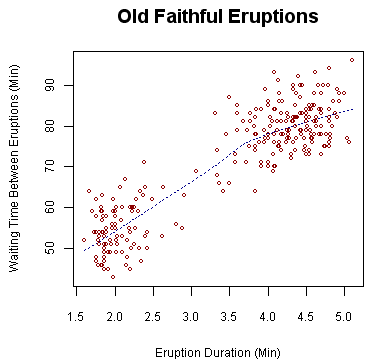
\includegraphics[width=0.5\textwidth]{c4.plot.scatter.01.png}
    \caption{Waiting time between eruptions and the duration of the eruption for the Old Faithful Geyser in Yellowstone National Park, Wyoming, USA. This chart suggests there are generally two ``types" of eruptions: short-wait-short-duration, and long-wait-long-duration.}
  \end{figure}
\end{frame}

\begin{frame}
  \frametitle{统计图形 | 气泡图}
  \begin{block}{气泡图}
    A bubble chart is a type of chart that displays three dimensions of data. Each entity with its triplet (v1, v2, v3) of associated data is plotted as a disk that expresses two of the vi values through the disk's xy location and the third through its size. Bubble charts can facilitate the understanding of social, economical, medical, and other scientific relationships.\\
    \vspace{0.5em}
Bubble charts can be considered a variation of the scatter plot, in which the data points are replaced with bubbles. As the documentation for Microsoft Office explains, ``You can use a bubble chart instead of a scatter chart if your data has three data series that each contain a set of values. The sizes of the bubbles are determined by the values in the third data series.".
  \end{block}
\end{frame}

\begin{frame}
  \frametitle{统计图形 | 气泡图}
  \begin{figure}
    \centering
    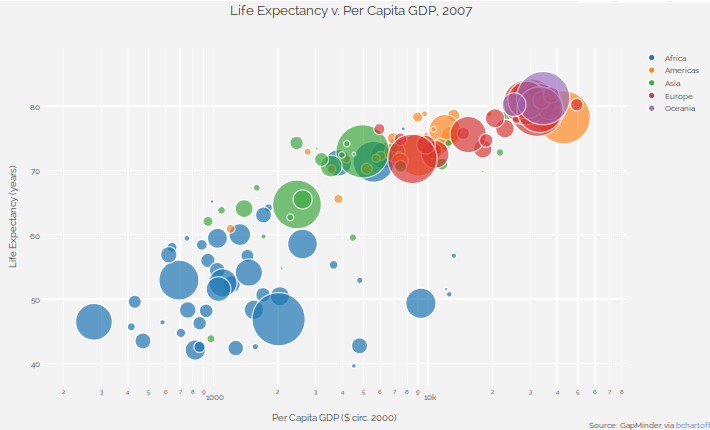
\includegraphics[width=0.9\textwidth]{c4.plot.bubble.01.png}
  \end{figure}
\end{frame}

\begin{frame}
  \frametitle{统计图形 | 折线图}
  \begin{block}{折线图}
    A line chart or line graph is a type of chart which displays information as a series of data points called `markers' connected by straight line segments.\\
    \vspace{0.5em}
    It is a basic type of chart common in many fields. It is similar to a scatter plot except that the measurement points are ordered (typically by their x-axis value) and joined with straight line segments.\\
    \vspace{0.5em}
    A line chart is often used to visualize a trend in data over intervals of time –\ a time series –\ thus the line is often drawn chronologically. In these cases they are known as run charts.
  \end{block}
\end{frame}

\begin{frame}
  \frametitle{统计图形 | 折线图}
  \begin{figure}
    \centering
    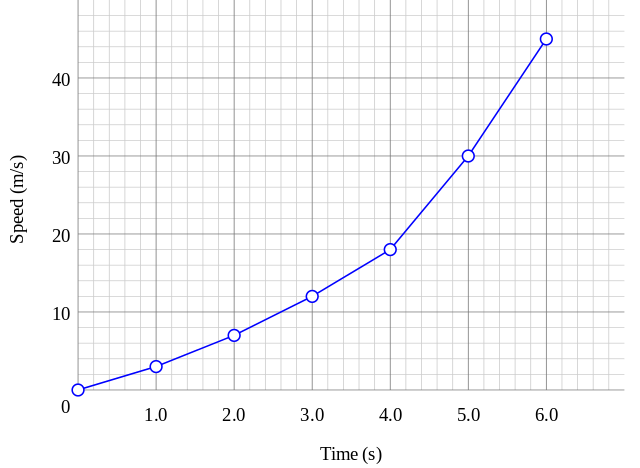
\includegraphics[width=0.9\textwidth]{c4.plot.linechart.01.png}
  \end{figure}
\end{frame}

\begin{frame}
  \frametitle{统计图形 | 趋势图}
  \begin{block}{趋势图}
    趋势图(run chart),也称运行图、链图、走势图,是一类在时间序列中表达数据变量的统计图表,通常该数据在一些工业或商业过程中可用来表达特定程序的表现。\\
    \vspace{0.5em}
    趋势图通常用于发现数据集中的异常现象,其暗示数据的变化往往是时间及其他特定因素所导致的变异性。\\
    \vspace{0.5em}
    A run chart, also known as a run-sequence plot is a graph that displays observed data in a time sequence. Often, the data displayed represent some aspect of the output or performance of a manufacturing or other business process. It is therefore a form of line chart.
  \end{block}
\end{frame}

% \begin{frame}
%   \frametitle{统计图形 | 趋势图}
%   \begin{figure}
%     \centering
%     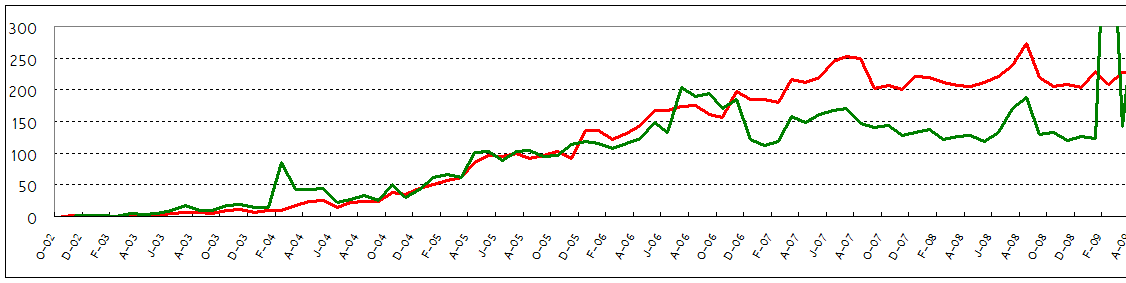
\includegraphics[width=0.9\textwidth]{c4.plot.runchart.01.png}
%   \end{figure}
% \end{frame}

\begin{frame}
  \frametitle{统计图形 | 趋势图}
  \begin{figure}
    \centering
    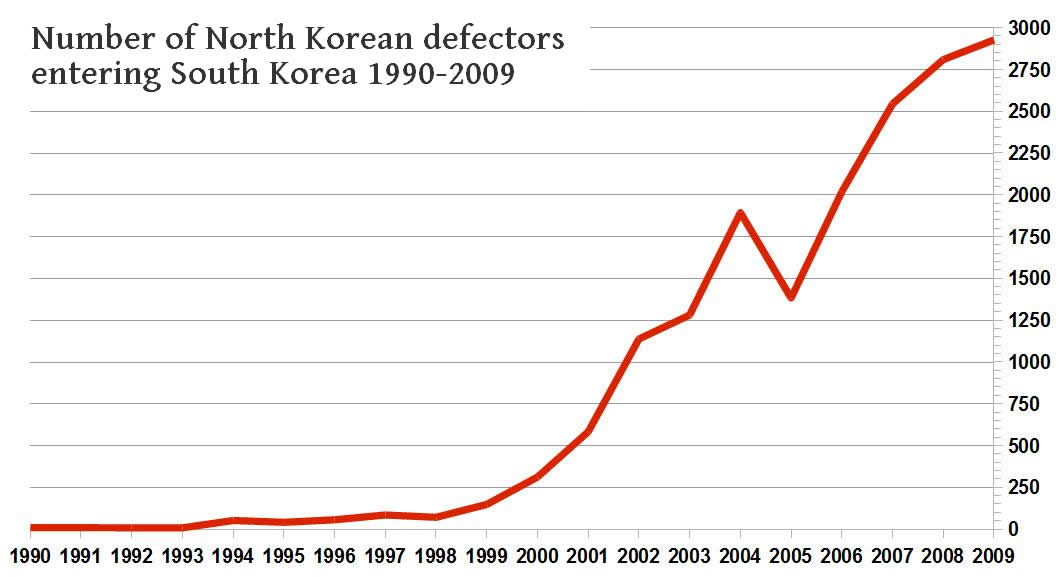
\includegraphics[width=0.9\textwidth]{c4.plot.runchart.02.jpg}
  \end{figure}
\end{frame}

\begin{frame}
  \frametitle{统计图形 | 概率图}
  \begin{block}{概率图}
    The normal probability plot is a graphical technique to identify substantive departures from normality. This includes identifying outliers, skewness, kurtosis, a need for transformations, and mixtures. Normal probability plots are made of raw data, residuals from model fits, and estimated parameters.\\
    \vspace{0.5em}
    In a normal probability plot (also called a "normal plot"), the sorted data are plotted vs. values selected to make the resulting image look close to a straight line if the data are approximately normally distributed. Deviations from a straight line suggest departures from normality.\\
    \vspace{0.5em}
The normal probability plot is a special case of the Q–Q probability plot for a normal distribution. The theoretical quantiles are generally chosen to approximate either the mean or the median of the corresponding order statistics.
  \end{block}
\end{frame}

\begin{frame}
  \frametitle{统计图形 | 概率图}
  \begin{figure}
    \centering
    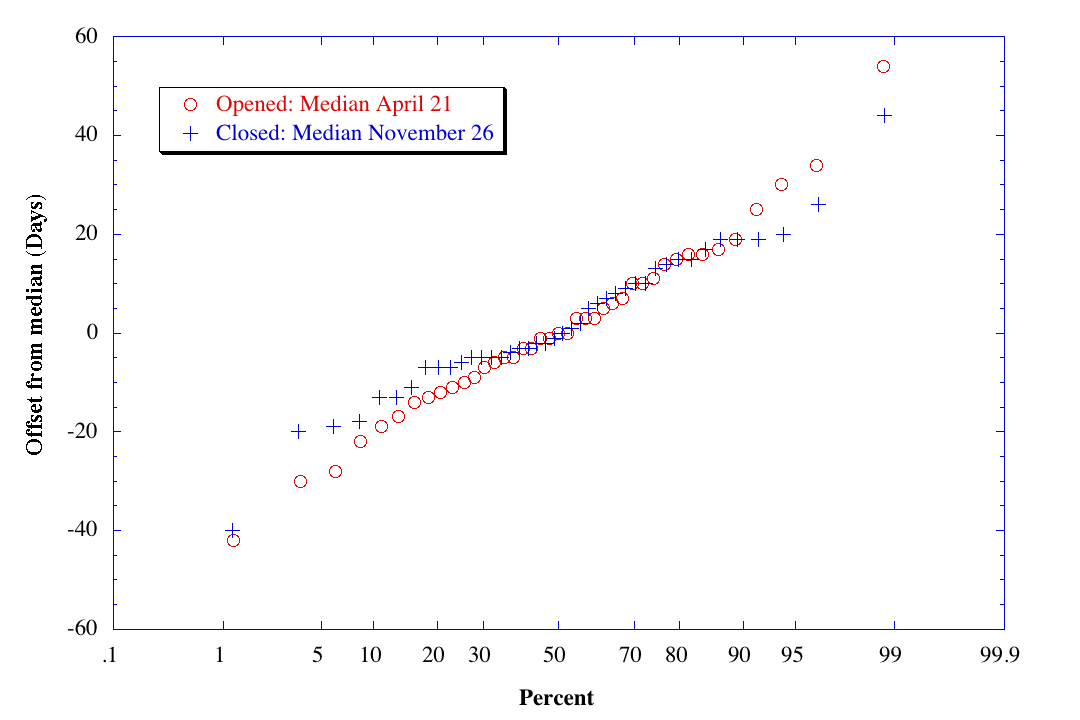
\includegraphics[width=0.85\textwidth]{c4.plot.qq.01.png}
    \caption{Q–Q plot for first opening/final closing dates of Washington State Route 20, versus a normal distribution. Outliers are visible in the upper right corner.}
  \end{figure}
\end{frame}

\begin{frame}
  \frametitle{统计图形 | 柱状图}
  \begin{block}{柱状图}
    长条图(bar chart)亦称条图(bar graph)、条状图、棒形图、柱状图,是一种以长方形的长度为变量的统计图表。长条图用来比较两个或以上的价值(不同时间或者不同条件),只有一个变量,通常用于较小的数据集分析。长条图亦可横向排列,或用多维方式表达。\\
%     \vspace{0.5em}
% 绘制长条图时,长条柱或柱组中线须对齐项目刻度。相较之下,折线图则是将数据代表之点对齐项目刻度。在数字大且接近时,两者皆可使用波浪形省略符号,以扩大表现数据间的差距,增强理解和清晰度。\\
\vspace{0.5em}
A bar chart or bar graph is a chart or graph that presents grouped data with rectangular bars with lengths proportional to the values that they represent. The bars can be plotted vertically or horizontally. A vertical bar chart is sometimes called a Line graph.\\
\vspace{0.5em}
A bar graph is a chart that uses either horizontal or vertical bars to show comparisons among categories. One axis of the chart shows the specific categories being compared, and the other axis represents a discrete value. Some bar graphs present bars clustered in groups of more than one.
  \end{block}
\end{frame}

\begin{frame}
  \frametitle{统计图形 | 柱状图}
  \begin{figure}
    \centering
    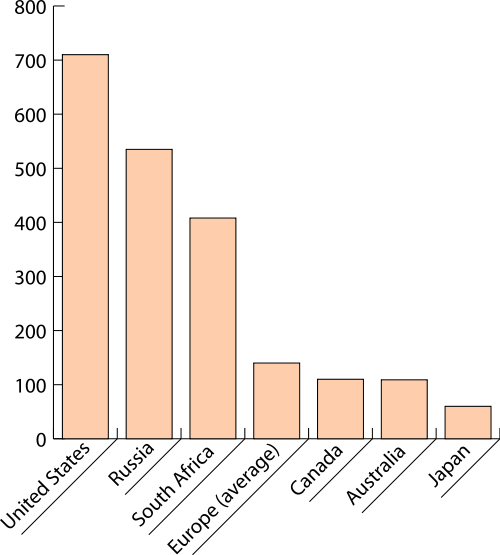
\includegraphics[width=0.4\textwidth]{c4.plot.barchart.01.png}
    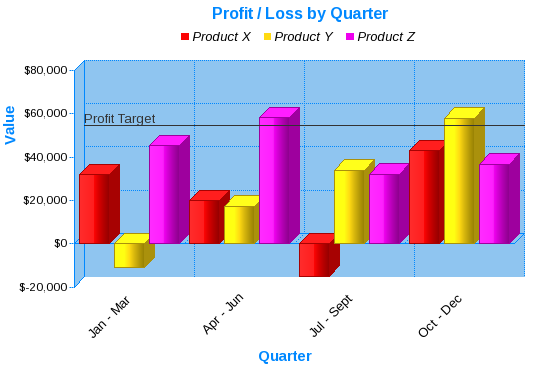
\includegraphics[width=0.55\textwidth]{c4.plot.barchart.02.png}
  \end{figure}
\end{frame}

\begin{frame}
  \frametitle{统计图形 | 柱状图}
  \begin{figure}
    \centering
    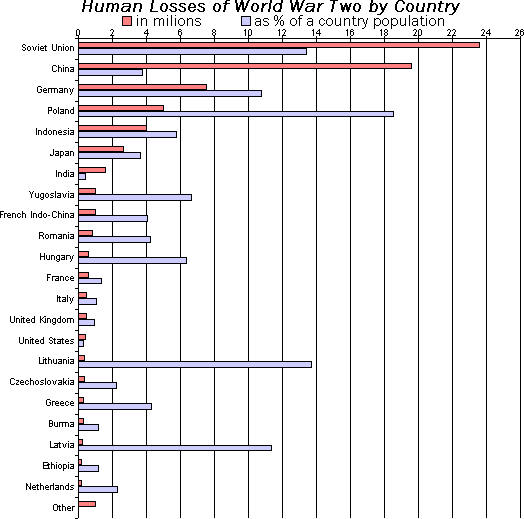
\includegraphics[width=0.65\textwidth]{c4.plot.barchart.03.png}
  \end{figure}
\end{frame}

\begin{frame}
  \frametitle{统计图形 | 直方图}
  \begin{block}{直方图}
在统计学中,直方图(Histogram)是一种对数据分布情况的图形表示,是一种二维统计图表,它的两个坐标分别是统计样本和该样本对应的某个属性的度量。直方图是品质管理七大工具之一。\\
    \vspace{0.5em}
    A histogram is a graphical representation of the distribution of numerical data. It is an estimate of the probability distribution of a continuous variable (quantitative variable) and was first introduced by Karl Pearson.It is a kind of bar graph.\\
    \vspace{0.5em}
    To construct a histogram, the first step is to ``bin" the range of values—that is, divide the entire range of values into a series of intervals—and then count how many values fall into each interval. The bins are usually specified as consecutive, non-overlapping intervals of a variable. The bins (intervals) must be adjacent, and are often (but are not required to be) of equal size.
  \end{block}
\end{frame}

\begin{frame}
  \frametitle{统计图形 | 直方图}
  \begin{figure}
    \centering
    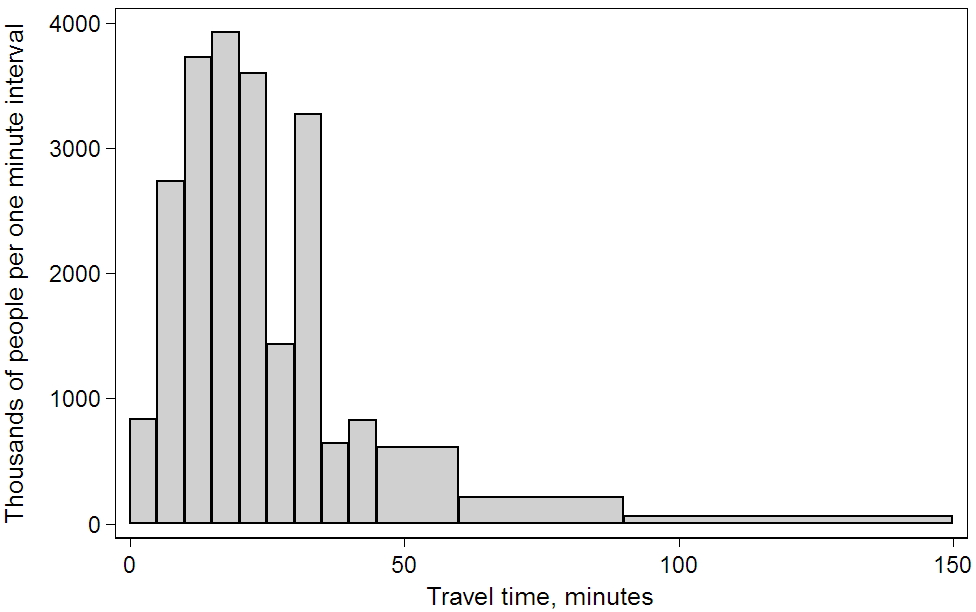
\includegraphics[width=0.9\textwidth]{c4.plot.histogram.01.png}
    \caption{Histogram of travel time (to work), US 2000 census. Area under the curve equals the total number of cases. This diagram uses Q/width from the table.}
  \end{figure}
\end{frame}

\begin{frame}
  \frametitle{统计图形 | 密度图}
  \begin{figure}
    \centering
    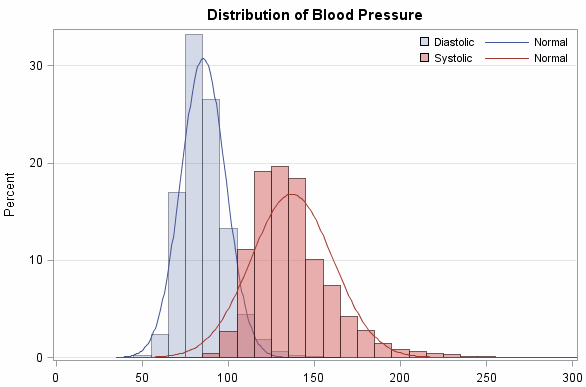
\includegraphics[width=0.9\textwidth]{c4.plot.density.01.png}
  \end{figure}
\end{frame}

\begin{frame}
  \frametitle{统计图形 | 茎叶图}
  \begin{block}{茎叶图}
%     茎叶图显示数据以说明其形状和分布。它与直方图相似。但是,茎叶图显示准确的数据点,从而使得计算均值、中位数和模式简便得多。\\
%     \vspace{0.5em}
% 在茎叶图中,每个数据值都分为“茎”和“叶”。“叶”通常是数字的最后一位,“叶”左侧的其他位形成“茎”。“叶单位”指明叶值代表的小数位。 图的每一行显示计数、茎和叶。中位数之前和之后的行计数是经过累积的。中位数前面一行的计数代表该行及其前面各行的总计数。中位数后面一行的计数代表该行及其后面各行的总计数。\\
% \vspace{0.5em}
% A stem-and-leaf display is a device for presenting quantitative data in a graphical format, similar to a histogram, to assist in visualizing the shape of a distribution. They evolved from Arthur Bowley's work in the early 1900s, and are useful tools in exploratory data analysis.\\
% \vspace{0.5em}
A stem-and-leaf display is often called a stemplot, but the latter term often refers to another chart type. A simple stem plot may refer to plotting a matrix of y values onto a common x axis, and identifying the common x value with a vertical line, and the individual y values with symbols on the line.\\
\vspace{0.5em}
Unlike histograms, stem-and-leaf displays retain the original data to at least two significant digits, and put the data in order, thereby easing the move to order-based inference and non-parametric statistics.\\
\vspace{0.5em}
A basic stem-and-leaf display contains two columns separated by a vertical line. The left column contains the stems and the right column contains the leaves.
  \end{block}
\end{frame}

\begin{frame}
  \frametitle{统计图形 | 茎叶图}
  \begin{figure}
    \centering
    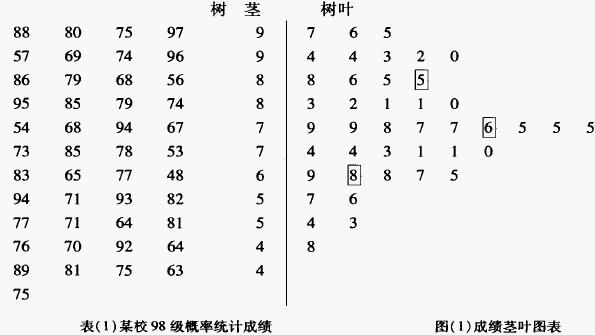
\includegraphics[width=0.55\textwidth]{c4.plot.stem.01.png}\\
    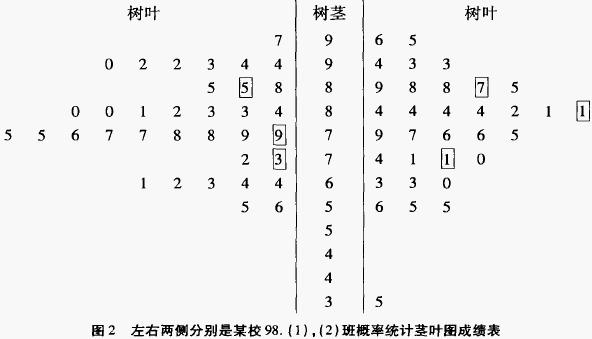
\includegraphics[width=0.55\textwidth]{c4.plot.stem.02.png}
  \end{figure}
\end{frame}

\begin{frame}
  \frametitle{统计图形 | 箱线图}
  \begin{block}{箱线图}
    箱形图(Box-plot),又称为盒须图、盒式图、盒状图或箱线图,是一种用作显示一组数据分散情况资料的统计图。因型状如箱子而得名。\\
    \vspace{0.5em}
箱形图于1977年由美国著名统计学家约翰·图基(John Tukey)发明。它能显示出一组数据的最大值、最小值、中位数、下四分位数及上四分位数。\\
\vspace{0.5em}
In descriptive statistics, a Box-Plot or Box-and-Whiskers-Diagram is a convenient way of graphically depicting groups of numerical data through their quartiles. Box plots may also have lines extending vertically from the boxes (whiskers) indicating variability outside the upper and lower quartiles, hence the terms box-and-whisker plot and box-and-whisker diagram. Outliers may be plotted as individual points. Box plots are non-parametric: they display variation in samples of a statistical population without making any assumptions of the underlying statistical distribution.
  \end{block}
\end{frame}

\begin{frame}
  \frametitle{统计图形 | 箱线图}
  \begin{figure}
    \centering
    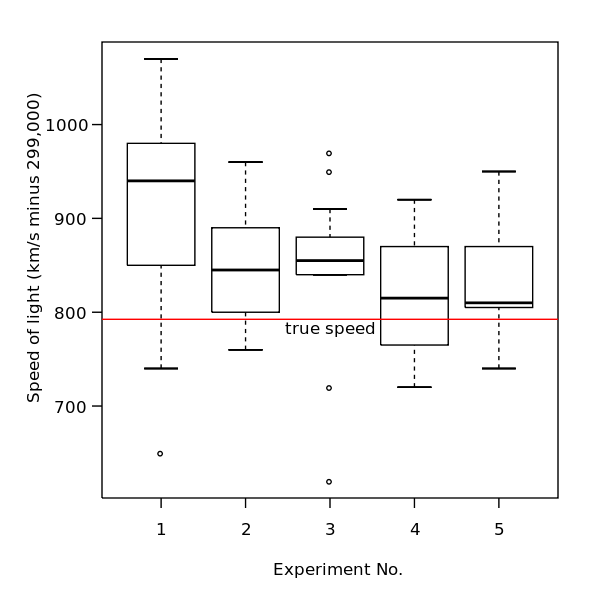
\includegraphics[width=0.6\textwidth]{c4.plot.boxplot.01.png}
    \caption{Box plot of data from the Michelson–Morley experiment.}
  \end{figure}
\end{frame}

\begin{frame}
  \frametitle{统计图形 | 箱线图}
  \begin{figure}
    \centering
    
\includegraphics[width=0.6\textwidth]{c4.plot.boxplot.02.png}
    \caption{Four box plots, with and without notches and variable width.}
  \end{figure}
\end{frame}

\begin{frame}
  \frametitle{统计图形 | 箱线图}
  \begin{figure}
    \centering
    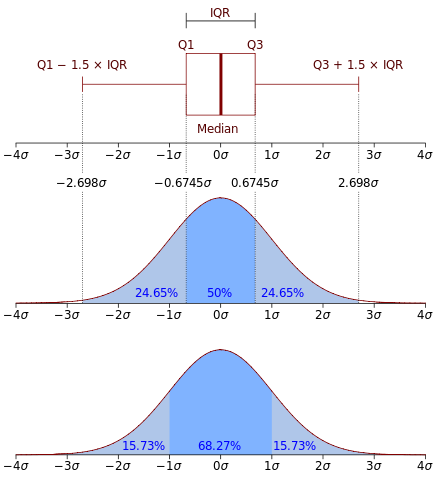
\includegraphics[width=0.5\textwidth]{c4.plot.boxplot.03.png}
    \caption{Boxplot and a probability density function (pdf) of a Normal $N(0,1\sigma^2)$ Population.}
  \end{figure}
\end{frame}

\begin{frame}
  \frametitle{统计图形 | 小提琴图}
  \begin{block}{小提琴图}
    {\footnotesize
    A violin plot is a method of plotting numeric data. It is similar to box plot with a rotated kernel density plot on each side.\\
    \vspace{0.5em}
The violin plot is similar to box plots, except that they also show the probability density of the data at different values (in the simplest case this could be a histogram). Typically violin plots will include a marker for the median of the data and a box indicating the interquartile range, as in standard box plots. Overlaid on this box plot is a kernel density estimation. Like box plots, violin plots are used to represent comparison of a variable distribution (or sample distribution) across different ``categories".\\
\vspace{0.5em}
A violin plot is more informative than a plain box plot. In fact while a box plot only shows summary statistics such as mean/median and interquartile ranges, the violin plot shows the full distribution of the data. The difference is particularly useful when the data distribution is multimodal (more than one peak). In this case a violin plot clearly shows the presence of different peaks, their position and relative amplitude. This information could not be represented with a simple box plot which only reports summary statistics. The inner part of a violin plot usually shows the mean (or median) and the interquartile range. In other cases, when the number of samples is not too high, the inner part can show all sample points (with a dot or a line for each sample).\\
    }
  \end{block}
\end{frame}

\begin{frame}
  \frametitle{统计图形 | 小提琴图}
  \begin{figure}
    \centering
    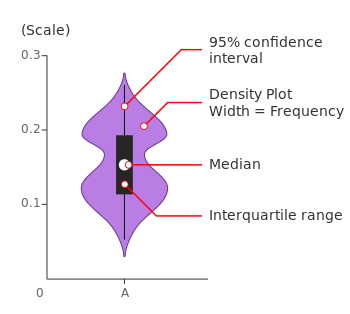
\includegraphics[width=0.45\textwidth]{c4.plot.violin.01.png}
    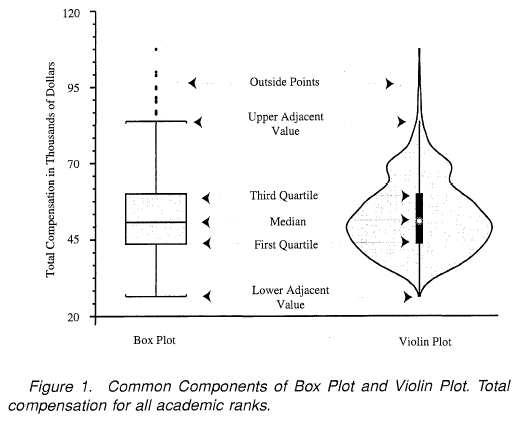
\includegraphics[width=0.45\textwidth]{c4.plot.violin.04.png}
  \end{figure}
\end{frame}

\begin{frame}
  \frametitle{统计图形 | 小提琴图}
  \begin{figure}
    \centering
    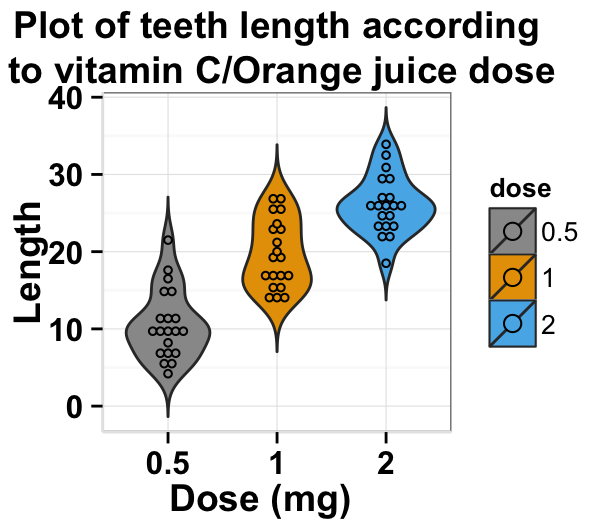
\includegraphics[width=0.45\textwidth]{c4.plot.violin.02.png}
    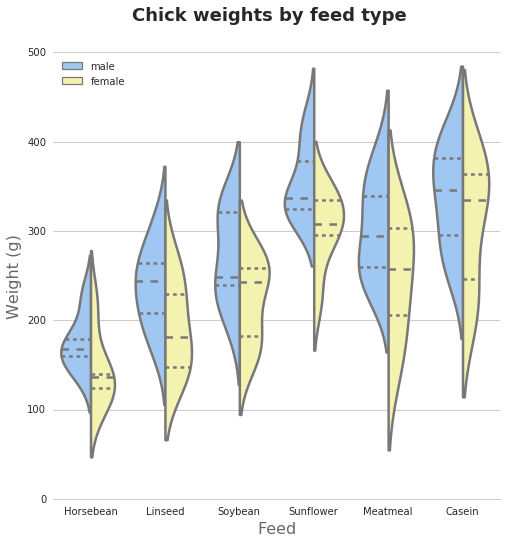
\includegraphics[width=0.45\textwidth]{c4.plot.violin.03.png}
  \end{figure}
\end{frame}

\begin{frame}
  \frametitle{统计图形 | 饼图}
  \begin{block}{饼图}
饼图,或称饼状图,是一个划分为几个扇形的圆形统计图表,用于描述量、频率或百分比之间的相对关系。在饼图中,每个扇区的弧长(以及圆心角和面积)大小为其所表示的数量的比例。这些扇区合在一起刚好是一个完全的圆形。顾名思义,这些扇区拼成了一个切开的饼形图案。\\
\vspace{1em}
饼图在商业领域和大众媒体中几乎无处不在,但很少用于科技出版物。这是受到批评最多的图表之一,而很多统计学家建议避免使用这一图表。它们指出,在饼图中很难对不同的扇区大小进行比较,或对不同饼图之间数据进行比较。\\
\vspace{0.5em}
在一些特定情况下,饼图可以很有效地对信息进行展示。特别是在想要表示某个大扇区在整体中所占比例,而不是对不同扇区进行比较时,这一方法十分有效。饼图在扇区所占比例达到总体的25\%或50\%时,可以很好地达到展示的目的。但通常,可能更多情况会采用其它图表如条形图或圆点图(dot plot),或非图表的方法如表格来表达信息。
  \end{block}
\end{frame}

\begin{frame}
  \frametitle{统计图形 | 饼图}
  \begin{figure}
    \centering
    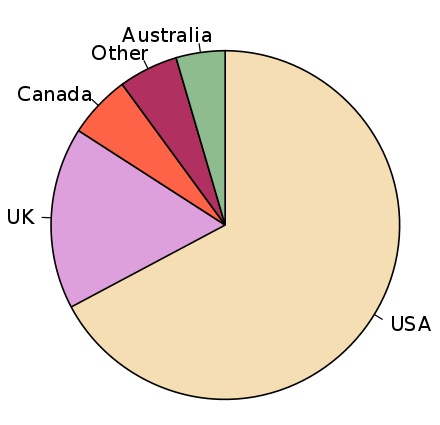
\includegraphics[width=0.6\textwidth]{c4.plot.pie.01.png}
    \caption{英语为母语的人口分布饼图。}
  \end{figure}
\end{frame}

\begin{frame}
  \frametitle{统计图形 | 饼图}
  \begin{figure}
    \centering
    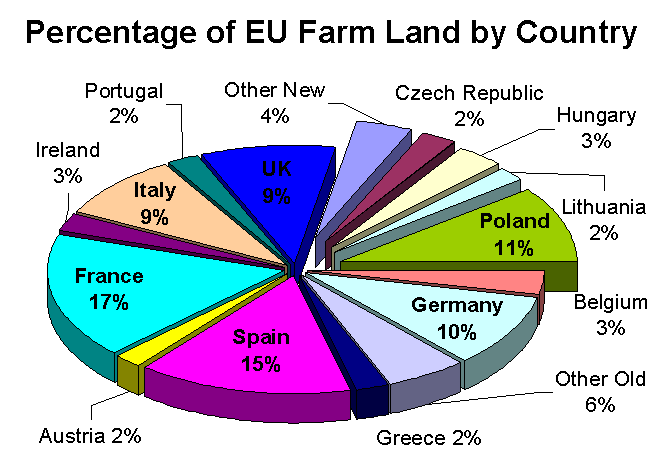
\includegraphics[width=0.85\textwidth]{c4.plot.pie.02.png}
    \caption{欧盟各国拥有欧盟农田的百分比。}
  \end{figure}
\end{frame}

\begin{frame}
  \frametitle{统计图形 | 韦恩图}
  \begin{block}{韦恩图}
    {\footnotesize
    文氏图(Venn diagram),或译Venn图、温氏图、维恩图、范氏图,是在所谓的集合论(或者类的理论)数学分支中,在不太严格的意义下用以表示集合(或类)的一种草图。它们用于展示在不同的事物群组(集合)之间的数学或逻辑联系,尤其适合用来表示集合(或)类之间的“大致关系”,它也常常被用来帮助推导(或理解推导过程)关于集合运算(或类运算)的一些规律。\\
    \vspace{0.5em}
    A Venn diagram (also called primary diagram, set diagram or logic diagram) is a diagram that shows all possible logical relations between a finite collection of different sets. These diagrams depict elements as points in the plane, and sets as regions inside closed curves. A Venn diagram consists of multiple overlapping closed curves, usually circles, each representing a set. The points inside a curve labelled S represent elements of the set S, while points outside the boundary represent elements not in the set S. In Venn diagrams the curves are overlapped in every possible way, showing all possible relations between the sets. They are thus a special case of Euler diagrams, which do not necessarily show all relations. Venn diagrams were conceived around 1880 by John Venn. They are used to teach elementary set theory, as well as illustrate simple set relationships in probability, logic, statistics, linguistics and computer science.\\
  }
  \end{block}
\end{frame}

\begin{frame}
  \frametitle{统计图形 | 韦恩图}
  \begin{figure}
    \centering
    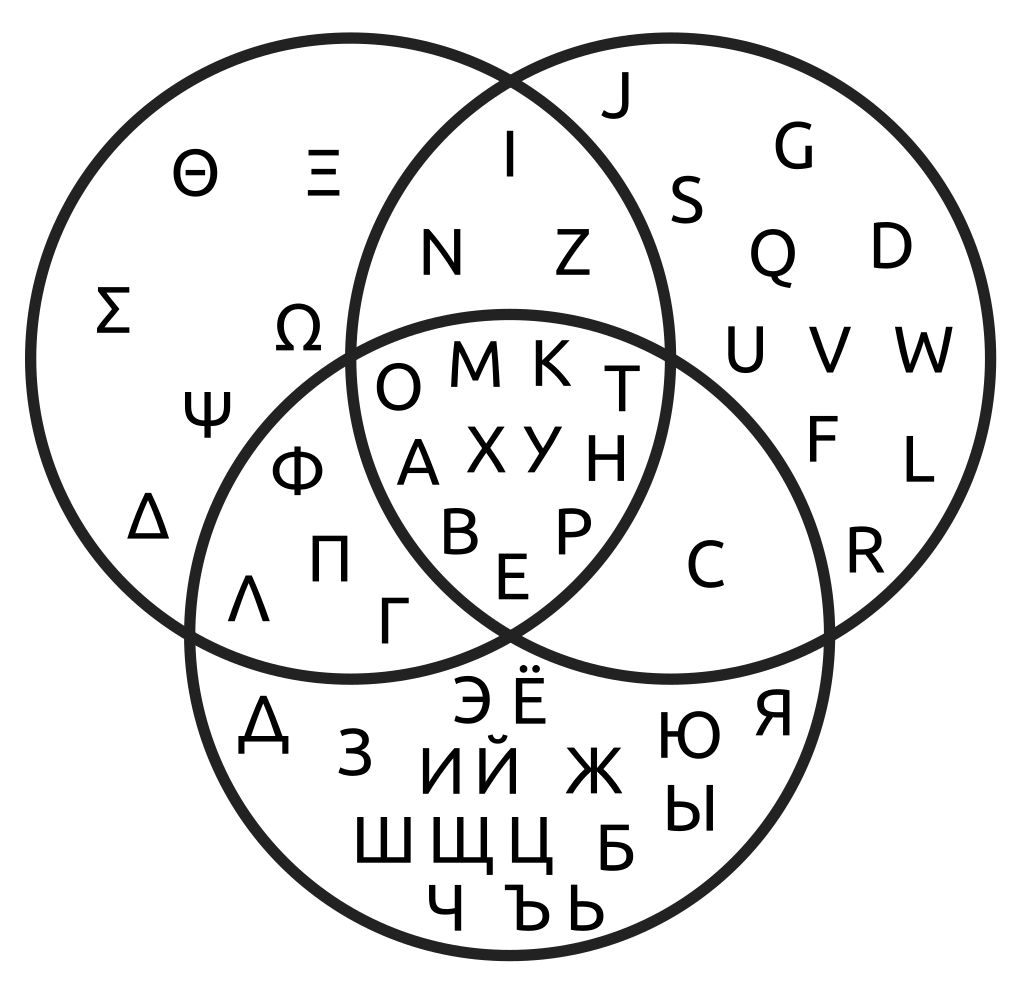
\includegraphics[width=0.45\textwidth]{c4.plot.venn.01.png}
    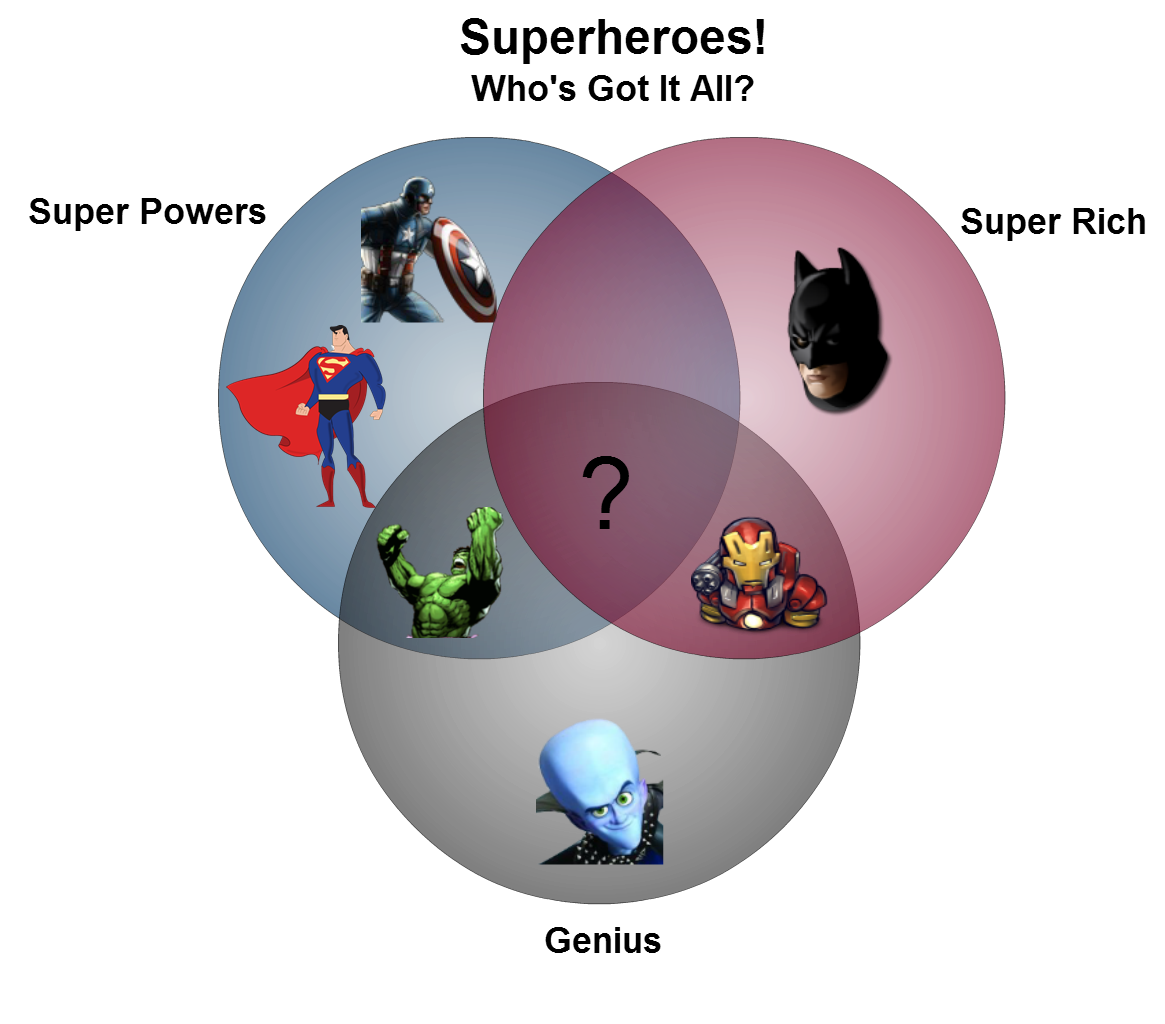
\includegraphics[width=0.55\textwidth]{c4.plot.venn.02.png}
  \end{figure}
\end{frame}

\begin{frame}
  \frametitle{统计图形 | 韦恩图}
  \begin{figure}
    \centering
    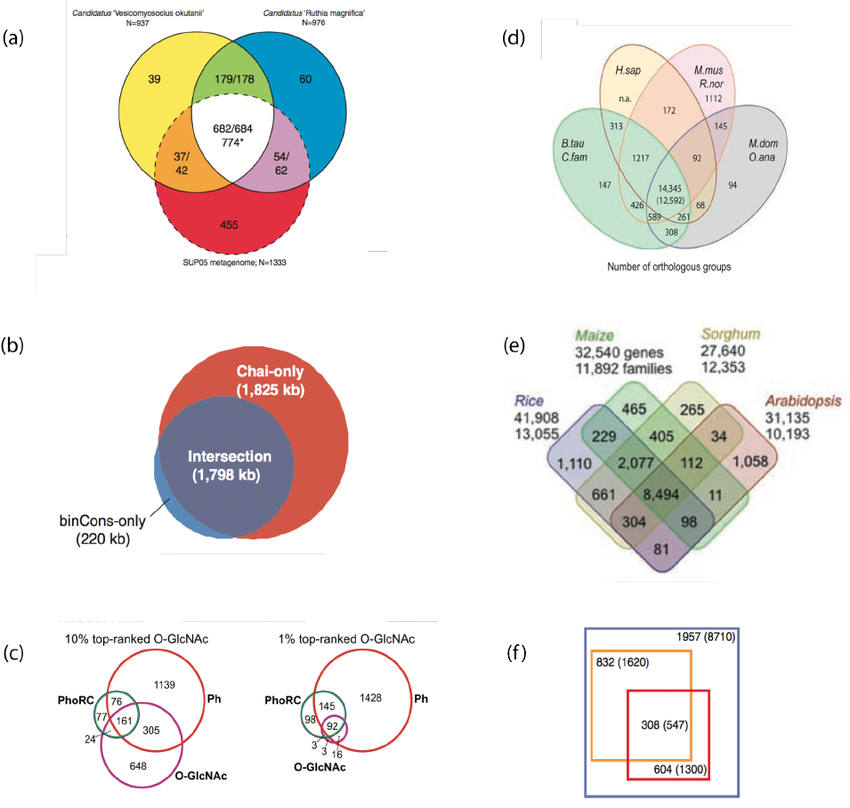
\includegraphics[width=0.7\textwidth]{c4.plot.venn.03.png}
  \end{figure}
\end{frame}

\begin{frame}
  \frametitle{统计图形 | 双标图}
  \begin{block}{双标图}
双标图(Biplots)是一类统计学的统计图形。双标图可以同时把抽样和资料矩阵变量中的数据用图表表示出来。抽样样本可以用向量、线性轴和非线性轨迹表达。在类别变量的案例中,类别水平点(category level points)可以用来代表其类别变量的水平值。一类广义的双标图可以适用呈现序数标量和区间标量。
  \end{block}
\end{frame}

\begin{frame}
  \frametitle{统计图形 | 双标图}
  \begin{figure}
    \centering
    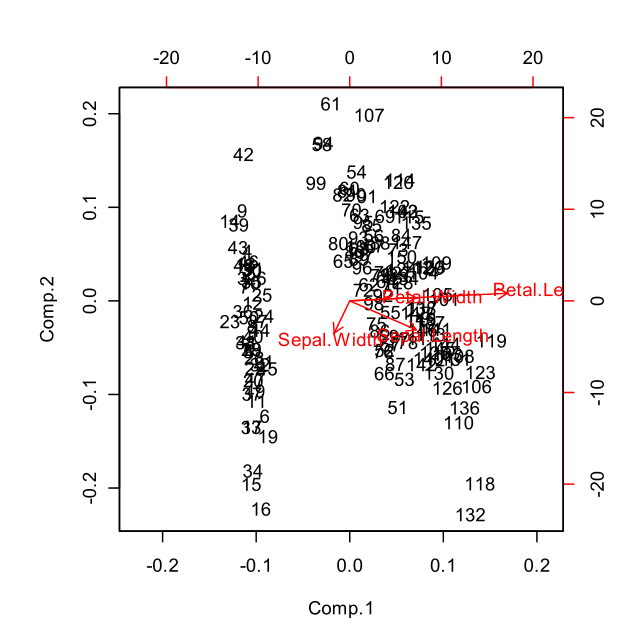
\includegraphics[width=0.6\textwidth]{c4.plot.biplot.01.png}
    \caption{Biplot of Anderson's iris data set.}
  \end{figure}
\end{frame}

\begin{frame}
  \frametitle{统计图形 | 雷达图}
  \begin{block}{雷达图}
    A radar chart is a graphical method of displaying multivariate data in the form of a two-dimensional chart of three or more quantitative variables represented on axes starting from the same point. The relative position and angle of the axes is typically uninformative.\\
    \vspace{0.5em}
The radar chart is also known as web chart, spider chart, star chart, star plot, cobweb chart, irregular polygon, polar chart, or Kiviat diagram. It is equivalent to a parallel coordinates plot in polar coordinates.
  \end{block}
\end{frame}

\begin{frame}
  \frametitle{统计图形 | 雷达图}
  \begin{figure}
    \centering
    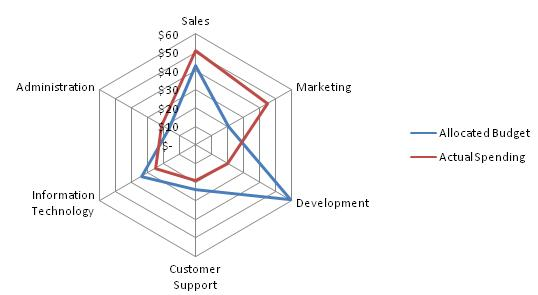
\includegraphics[width=0.9\textwidth]{c4.plot.star.02.jpg}
    \caption{This spider chart represents the allocated budget versus actual spending for a given organization.}
  \end{figure}
\end{frame}

\begin{frame}
  \frametitle{统计图形 | 雷达图}
  \begin{figure}
    \centering
    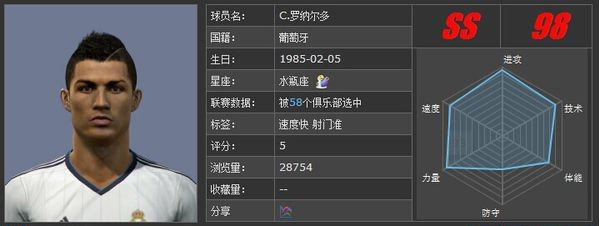
\includegraphics[width=0.6\textwidth]{c4.plot.star.03.jpg}\\
    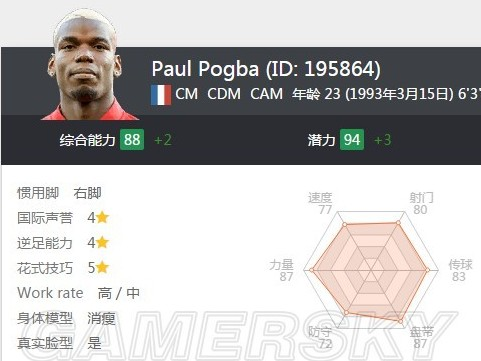
\includegraphics[width=0.6\textwidth]{c4.plot.star.05.jpg}
  \end{figure}
\end{frame}

\begin{frame}
  \frametitle{统计图形 | 森林图}
  \begin{block}{森林图}
    A forest plot, also known as a blobbogram, is a graphical display of estimated results from a number of scientific studies addressing the same question, along with the overall results.\\
    \vspace{0.5em}
It was developed for use in medical research as a means of graphically representing a meta-analysis of the results of randomized controlled trials. In the last twenty years, similar meta-analytical techniques have been applied in observational studies (e.g. environmental epidemiology) and forest plots are often used in presenting the results of such studies also.
  \end{block}
\end{frame}

\begin{frame}
  \frametitle{统计图形 | 森林图}
  \begin{figure}
    \centering
    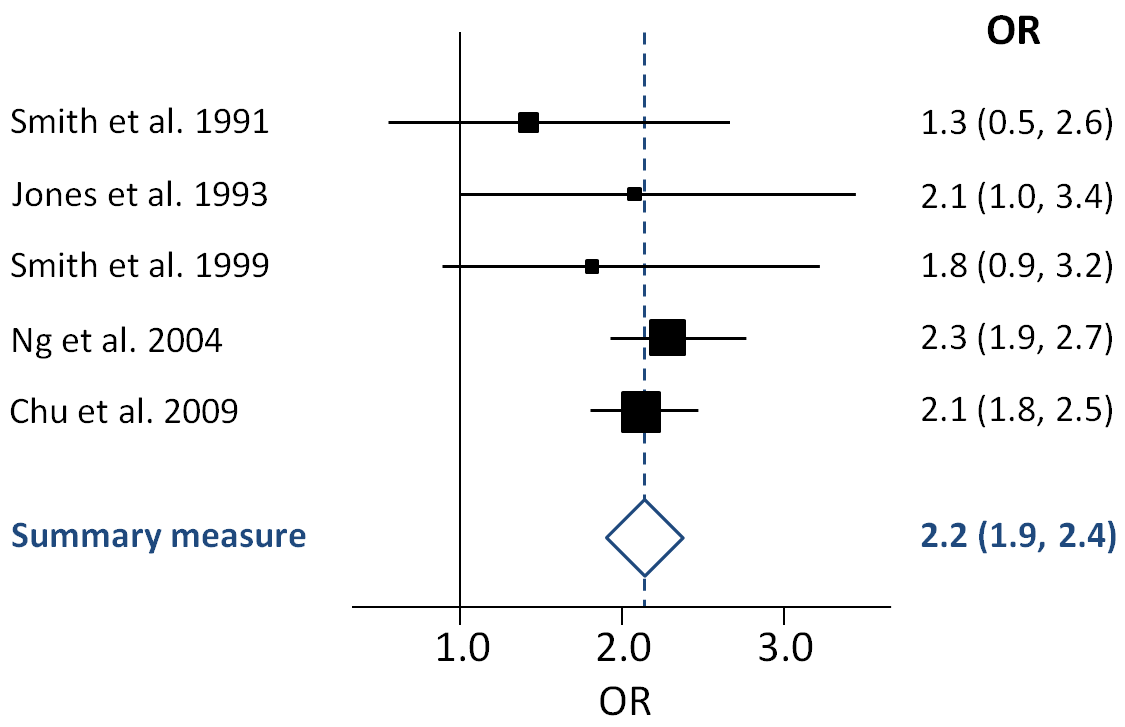
\includegraphics[width=0.7\textwidth]{c4.plot.forest.01.png}
    \caption{An example forest plot of five odds ratios (squares, proportional to weights used in meta-analysis), with the summary measure (centre line of diamond) and associated confidence intervals (lateral tips of diamond), and solid vertical line of no effect. Names of (fictional) studies are shown on the left, odds ratios and confidence intervals on the right.}
  \end{figure}
\end{frame}

\begin{frame}
  \frametitle{统计图形 | 热图}
  \begin{block}{热图}
    A heat map (or heatmap) is a graphical representation of data where the individual values contained in a matrix are represented as colors. The term `heat map' was originally coined and trademarked by software designer Cormac Kinney in 1991, to describe a 2D display depicting financial market information, though similar plots such as shading matrices have existed for over a century.
  \end{block}
\end{frame}

\begin{frame}
  \frametitle{统计图形 | 热图}
  \begin{figure}
    \centering
    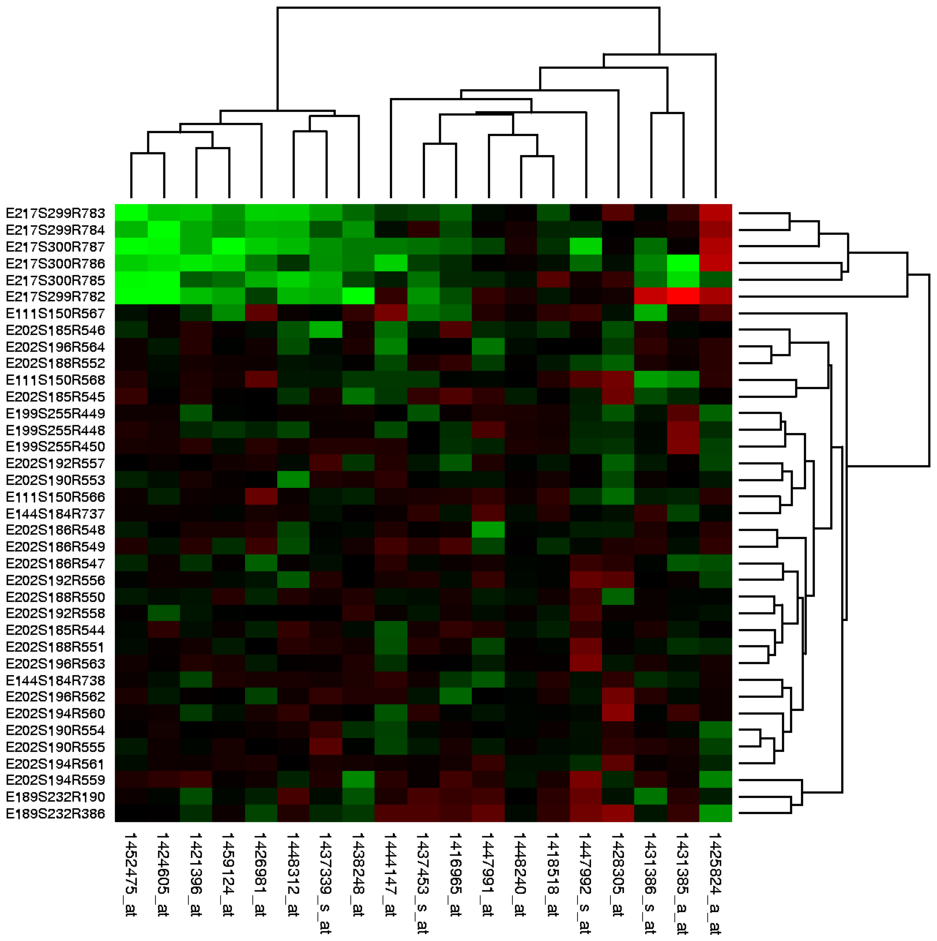
\includegraphics[width=0.55\textwidth]{c4.plot.heatmap.01.png}
    \caption{Heat map generated from DNA microarray data reflecting gene expression values in several conditions.}
  \end{figure}
\end{frame}

\begin{frame}
  \frametitle{统计图形 | 火山图}
  \begin{block}{火山图}
    {\footnotesize
    In statistics, a volcano plot is a type of scatter-plot that is used to quickly identify changes in large data sets composed of replicate data. It plots significance versus fold-change on the y and x axes, respectively. These plots are increasingly common in omic experiments such as genomics, proteomics, and metabolomics where one often has a list of many thousands of replicate data points between two conditions and one wishes to quickly identify the most meaningful changes. A volcano plot combines a measure of statistical significance from a statistical test (e.g., a p value from an ANOVA model) with the magnitude of the change, enabling quick visual identification of those data-points (genes, etc.) that display large magnitude changes that are also statistically significant.\\
    \vspace{0.5em}
A volcano plot is constructed by plotting the negative log of the p value on the y axis (usually base 10). This results in data points with low p values (highly significant) appearing toward the top of the plot. The x axis is the log of the fold change between the two conditions. The log of the fold change is used so that changes in both directions appear equidistant from the center. Plotting points in this way results in two regions of interest in the plot: those points that are found toward the top of the plot that are far to either the left- or right-hand sides. These represent values that display large magnitude fold changes (hence being left or right of center) as well as high statistical significance (hence being toward the top).\\
    }
  \end{block}
\end{frame}

\begin{frame}
  \frametitle{统计图形 | 火山图}
  \begin{figure}
    \centering
    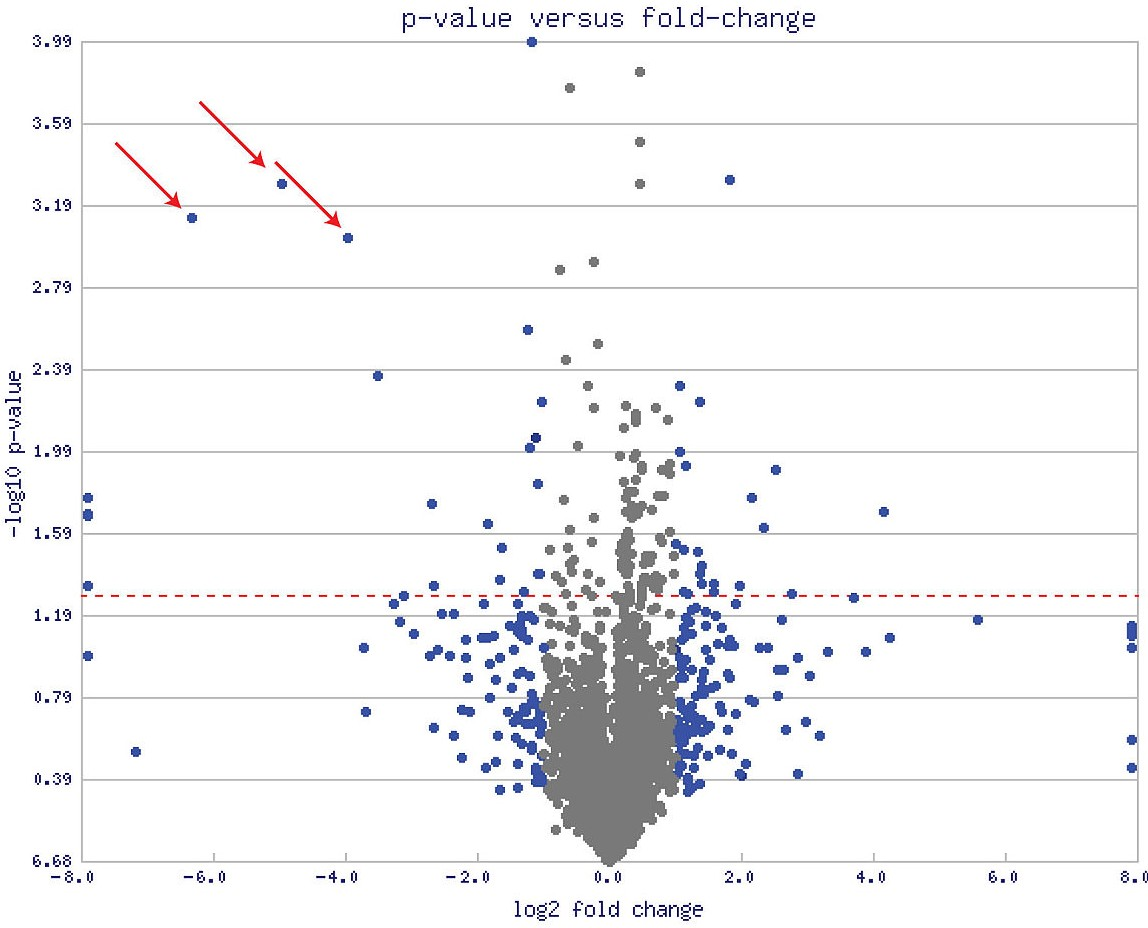
\includegraphics[width=0.6\textwidth]{c4.plot.volcano.01.jpg}
    \caption{{\scriptsize Volcano plot showing metabolomic data. The red arrows indicate points-of-interest that display both large magnitude fold-changes (x axis) and high statistical significance (-log10 of p value, y axis). The dashed red line shows where p = 0.05 with points above the line having p < 0.05 and points below the line having p > 0.05. This plot is colored such that those points having a fold-change less than 2 (log2 = 1) are shown in gray.\\ }}
  \end{figure}
\end{frame}

\begin{frame}
  \frametitle{统计图形 | 曼哈顿图}
  \begin{block}{曼哈顿图}
    A Manhattan plot is a type of scatter plot, usually used to display data with a large number of data-points - many of non-zero amplitude, and with a distribution of higher-magnitude values, for instance in genome-wide association studies (GWAS). In GWAS Manhattan plots, genomic coordinates are displayed along the X-axis, with the negative logarithm of the association P-value for each single nucleotide polymorphism (SNP) displayed on the Y-axis, meaning that each dot on the Manhattan plot signifies a SNP. Because the strongest associations have the smallest P-values (e.g., $10^{-15}$), their negative logarithms will be the greatest (e.g., 15).
  \end{block}
\end{frame}

\begin{frame}
  \frametitle{统计图形 | 曼哈顿图}
  \begin{figure}
    \centering
    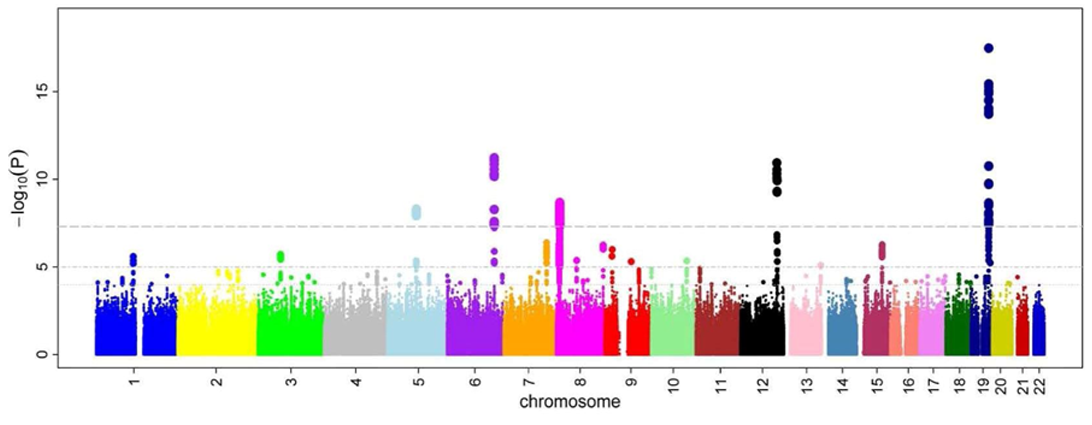
\includegraphics[width=\textwidth]{c4.plot.manhattan.01.png}
    \caption{An illustration of a Manhattan plot depicting several strongly associated risk loci.}
  \end{figure}
\end{frame}

\begin{frame}
  \frametitle{统计图形 | 网络可视化}
  \begin{block}{网络可视化}
Graph drawing is an area of mathematics and computer science combining methods from geometric graph theory and information visualization to derive two-dimensional depictions of graphs arising from applications such as social network analysis, cartography, linguistics, and bioinformatics.\\
\vspace{0.3em}
A drawing of a graph or network diagram is a pictorial representation of the vertices and edges of a graph. This drawing should not be confused with the graph itself: very different layouts can correspond to the same graph. In the abstract, all that matters is which pairs of vertices are connected by edges. In the concrete, however, the arrangement of these vertices and edges within a drawing affects its understandability, usability, fabrication cost, and aesthetics. The problem gets worse, if the graph changes over time by adding and deleting edges (dynamic graph drawing) and the goal is to preserve the user's mental map.
  \end{block}
\end{frame}

\begin{frame}
  \frametitle{统计图形 | 网络可视化}
  \begin{figure}
    \centering
    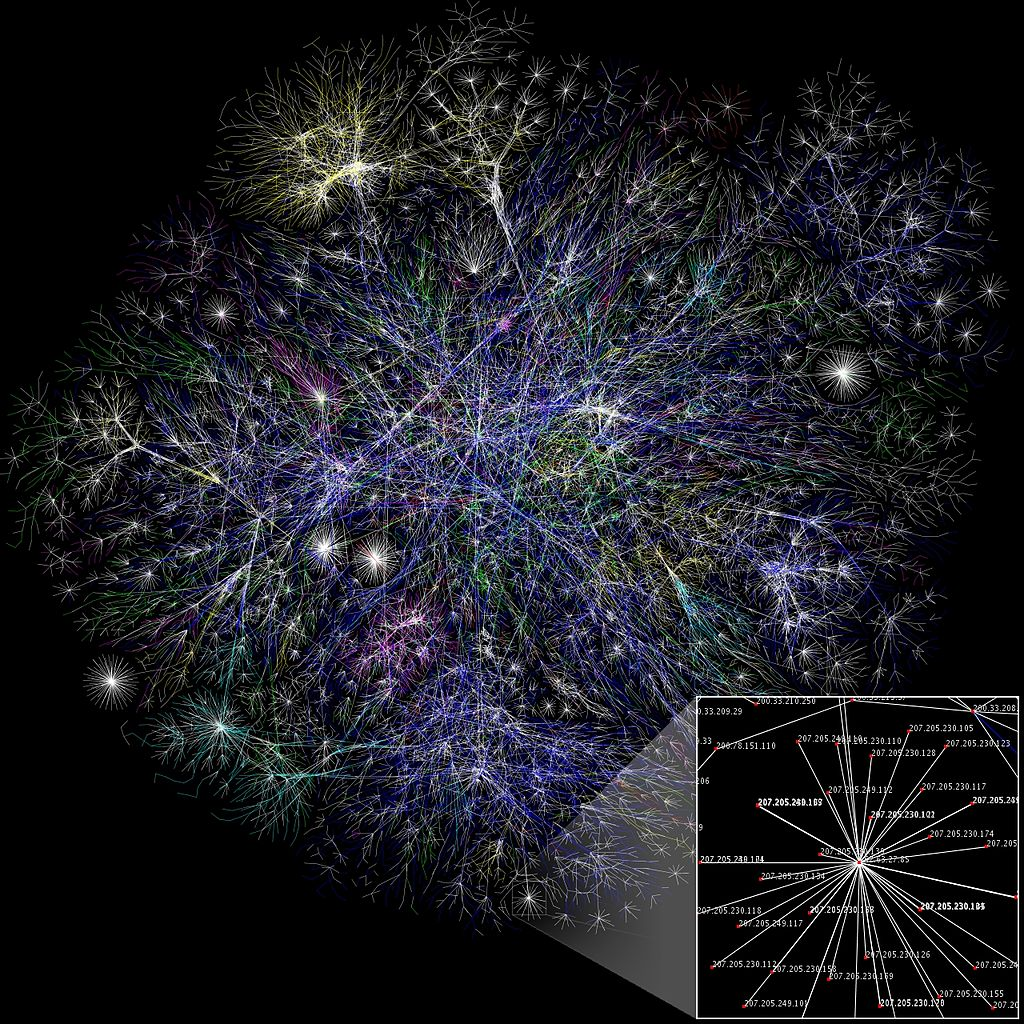
\includegraphics[width=0.6\textwidth]{c4.plot.network.01.jpg}
    \caption{{\footnotesize 2005年初因特网的部分映射,每条线表示两个IP地址以及两个节点之间的延迟。}}
  \end{figure}
\end{frame}

\begin{frame}
  \frametitle{统计图形 | 矩形树图}
  \begin{block}{矩形树图}
    In information visualization and computing, treemapping is a method for displaying hierarchical data using nested rectangles.\\
    \vspace{0.5em}
Treemaps display hierarchical (tree-structured) data as a set of nested rectangles. Each branch of the tree is given a rectangle, which is then tiled with smaller rectangles representing sub-branches. A leaf node's rectangle has an area proportional to a specified dimension of the data. Often the leaf nodes are colored to show a separate dimension of the data.\\
\vspace{0.5em}
When the color and size dimensions are correlated in some way with the tree structure, one can often easily see patterns that would be difficult to spot in other ways, such as if a certain color is particularly relevant. A second advantage of treemaps is that, by construction, they make efficient use of space. As a result, they can legibly display thousands of items on the screen simultaneously.
  \end{block}
\end{frame}

\begin{frame}
  \frametitle{统计图形 | 矩形树图}
  \begin{figure}
    \centering
    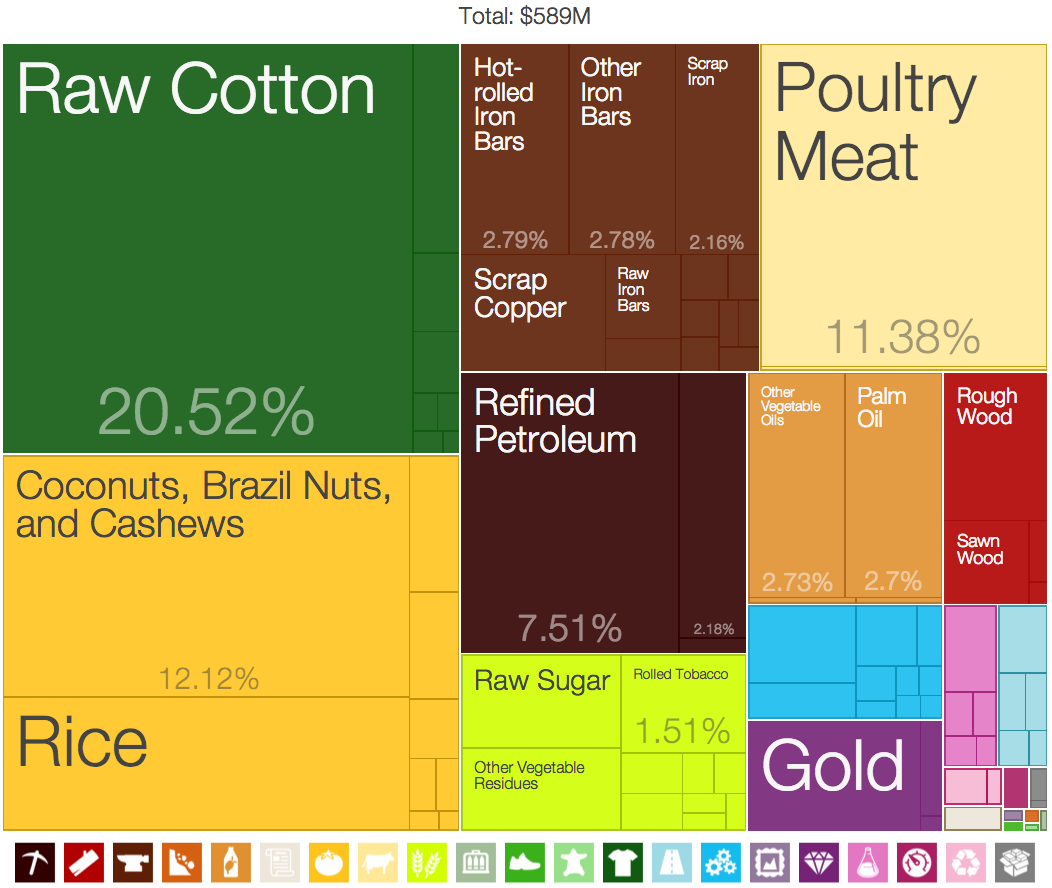
\includegraphics[width=0.65\textwidth]{c4.plot.treemap.03.png}
    \caption{{\footnotesize Treemap of Benin's exports by product category, 2009. The Product Exports Treemaps are one of the most recent applications of these kind of visualizations, developed by the Harvard-MIT Observatory of Economic Complexity.}}
  \end{figure}
\end{frame}

\begin{frame}
  \frametitle{统计图形 | 示意地图}
  \begin{block}{示意地图}
示意地图(Cartogram),又称比较统计地图,是将地图根据统计数据变形得到示意图,通常是将各个地理单位的面积扩大或缩小,来表示有关数据的数值。\\
\vspace{0.5em}
示意地图的用途在于视觉上展示统计数据,在尽可能保持各数据点之间的相对位置之时,亦透过数据点的实际面积来标示其数值,使读者不会因为地理因素影响而产生错觉。
  \end{block}
  \pause
  \begin{block}{实例}
2004年美国总统选举的投票分布图,若以传统的地理图表显示,会看到小布什得到压倒性的支持。不过,一旦用示意地图把同一组数据重组,就会发现原来因为大多数支持民主党的支持者都集中在沿岸的大城市,所以在地理图中被挤至边沿。事实上,双方的确是势均力敌的。
  \end{block}
\end{frame}

\begin{frame}
  \frametitle{统计图形 | 示意地图}
  \begin{figure}
    \centering
    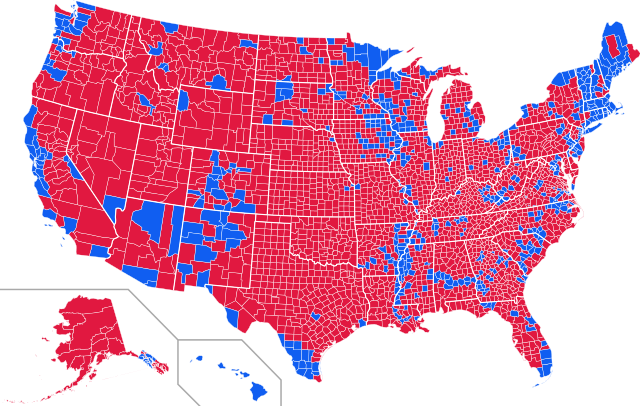
\includegraphics[width=0.45\textwidth]{c4.plot.cartogram.00.png}
    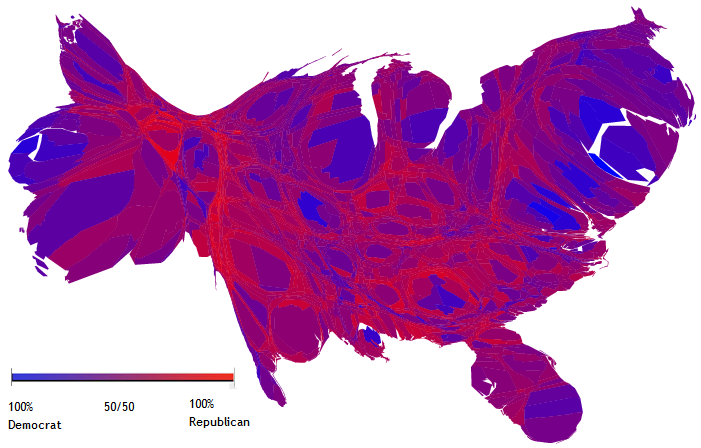
\includegraphics[width=0.45\textwidth]{c4.plot.cartogram.02.png}
  \end{figure}
\end{frame}

\begin{frame}
  \frametitle{统计图形 | 示意地图}
  \begin{figure}
    \centering
    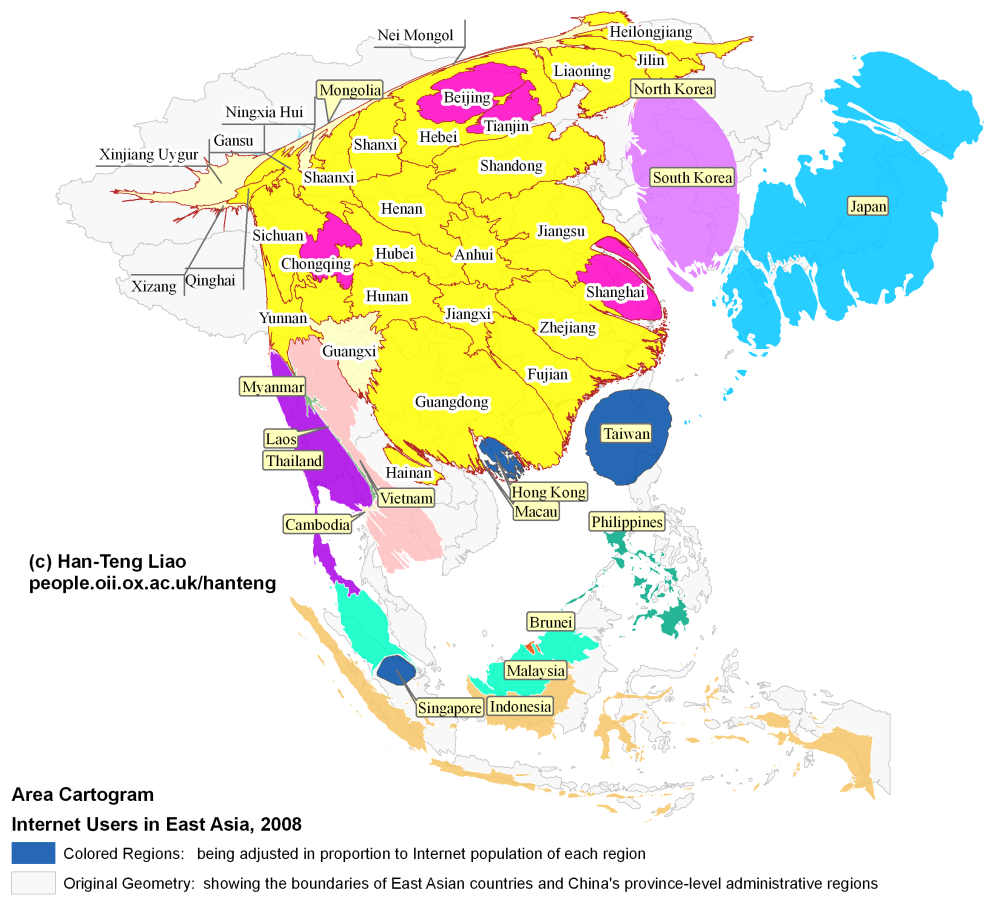
\includegraphics[width=0.65\textwidth]{c4.plot.cartogram.03.png}
    \caption{2008年东亚网民分布的面积统计比较地图,面积愈大代表人数愈多。}
  \end{figure}
\end{frame}

\begin{frame}
  \frametitle{统计图形 | 总结}
  \begin{figure}
    \centering
    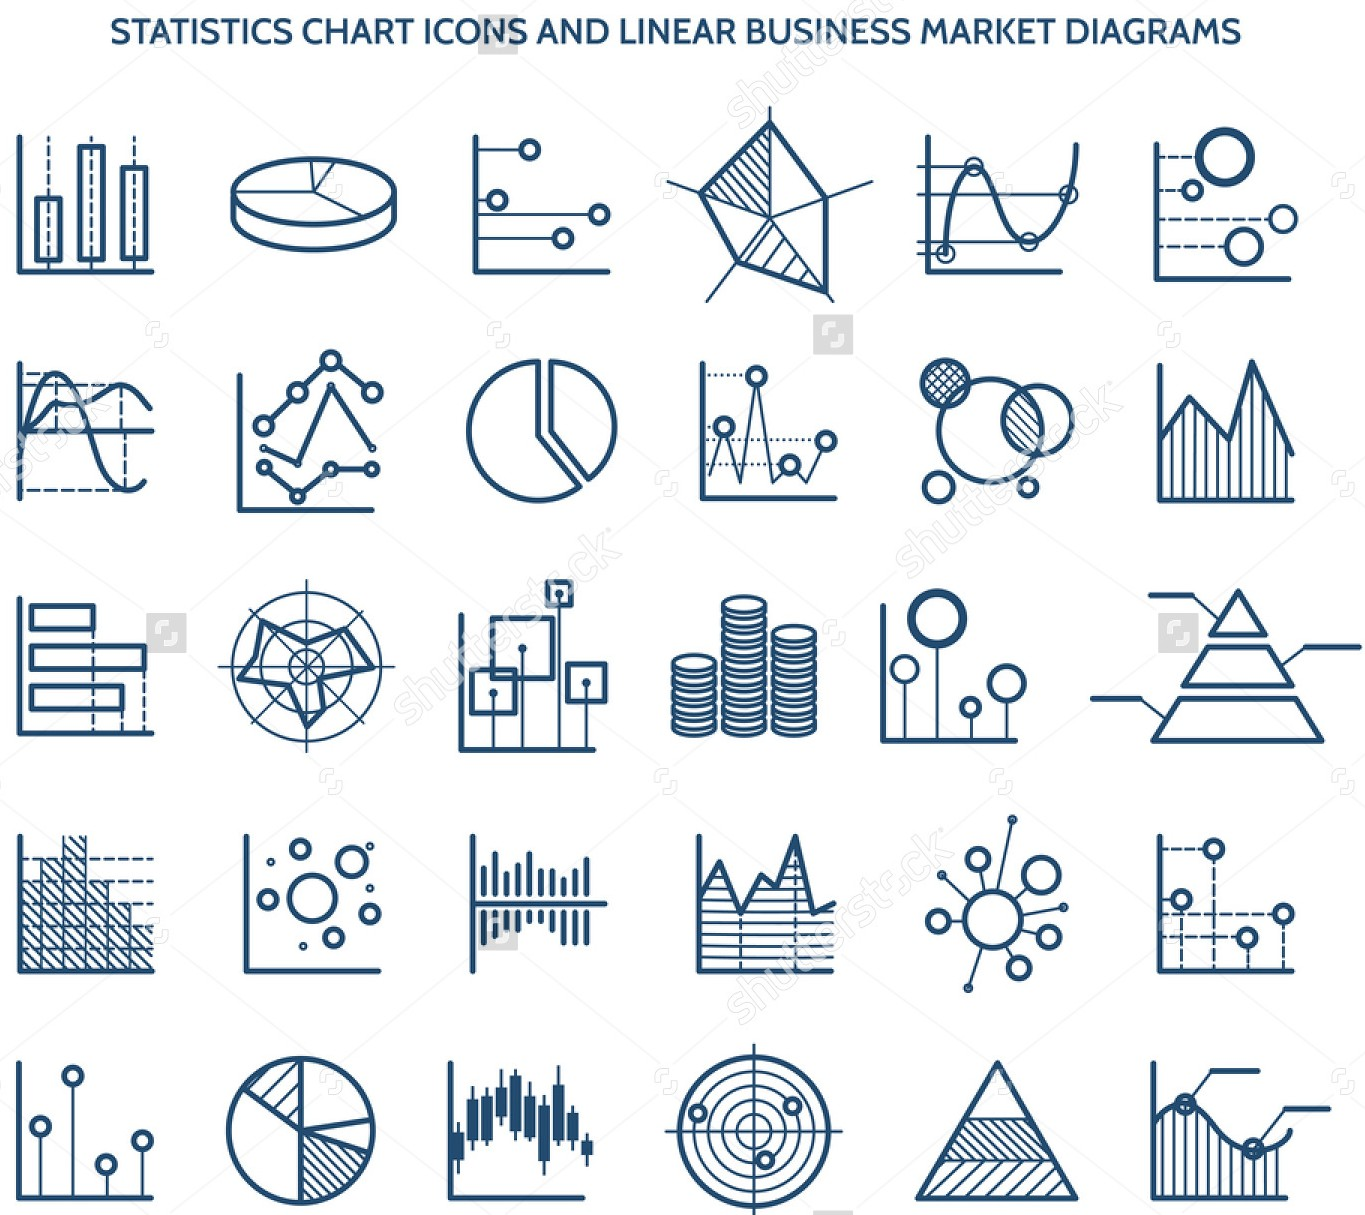
\includegraphics[width=0.7\textwidth]{c4.plot.all.01.jpg}
  \end{figure}
\end{frame}

\subsection{著名设计者}
\begin{frame}
  \frametitle{统计图形 | 设计者 | 威廉·普莱费尔}
  \begin{block}{威廉·普莱费尔(William Playfair)}
    发表了所谓的第一幅饼图以及众所周知的那张描绘英格兰进出口发展演变情况的图形。\\
    \vspace{0.5em}
    William Playfair was a Scottish engineer and political economist, the founder of graphical methods of statistics.\\
    \vspace{0.5em}
    William Playfair invented several types of diagrams: in 1786 the line, area and bar chart of economic data, and in 1801 the pie chart and circle graph, used to show part-whole relations.
  \end{block}
\end{frame}

\begin{frame}
  \frametitle{统计图形 | 设计者 | 威廉·普莱费尔}
  \begin{figure}
    \centering
    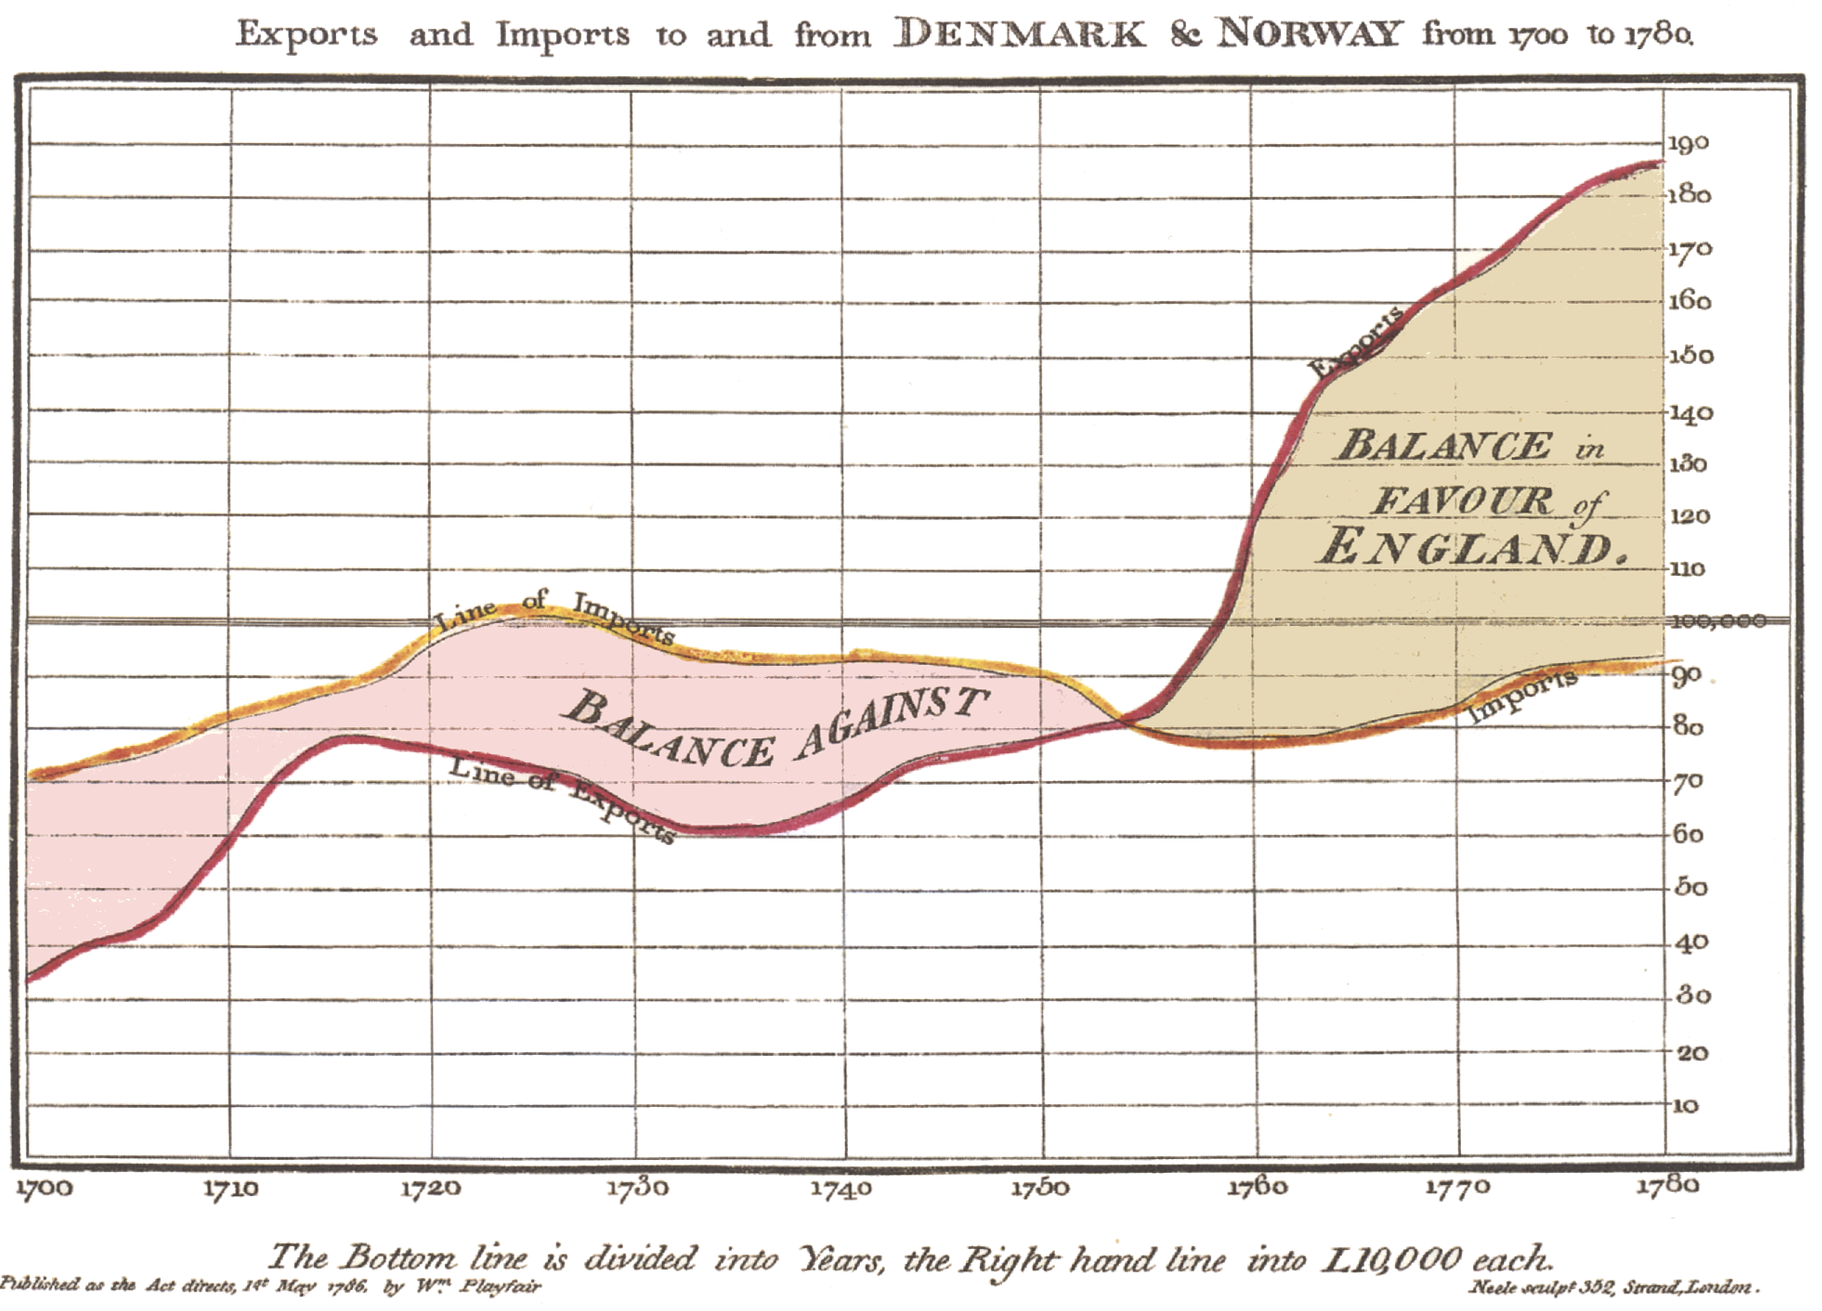
\includegraphics[width=0.9\textwidth]{c4.playfair.01.png}
    \caption{Playfair's trade-balance time-series chart, published in his Commercial and Political Atlas, 1786.}
  \end{figure}
\end{frame}

\begin{frame}
  \frametitle{统计图形 | 设计者 | 威廉·普莱费尔}
  \begin{figure}
    \centering
    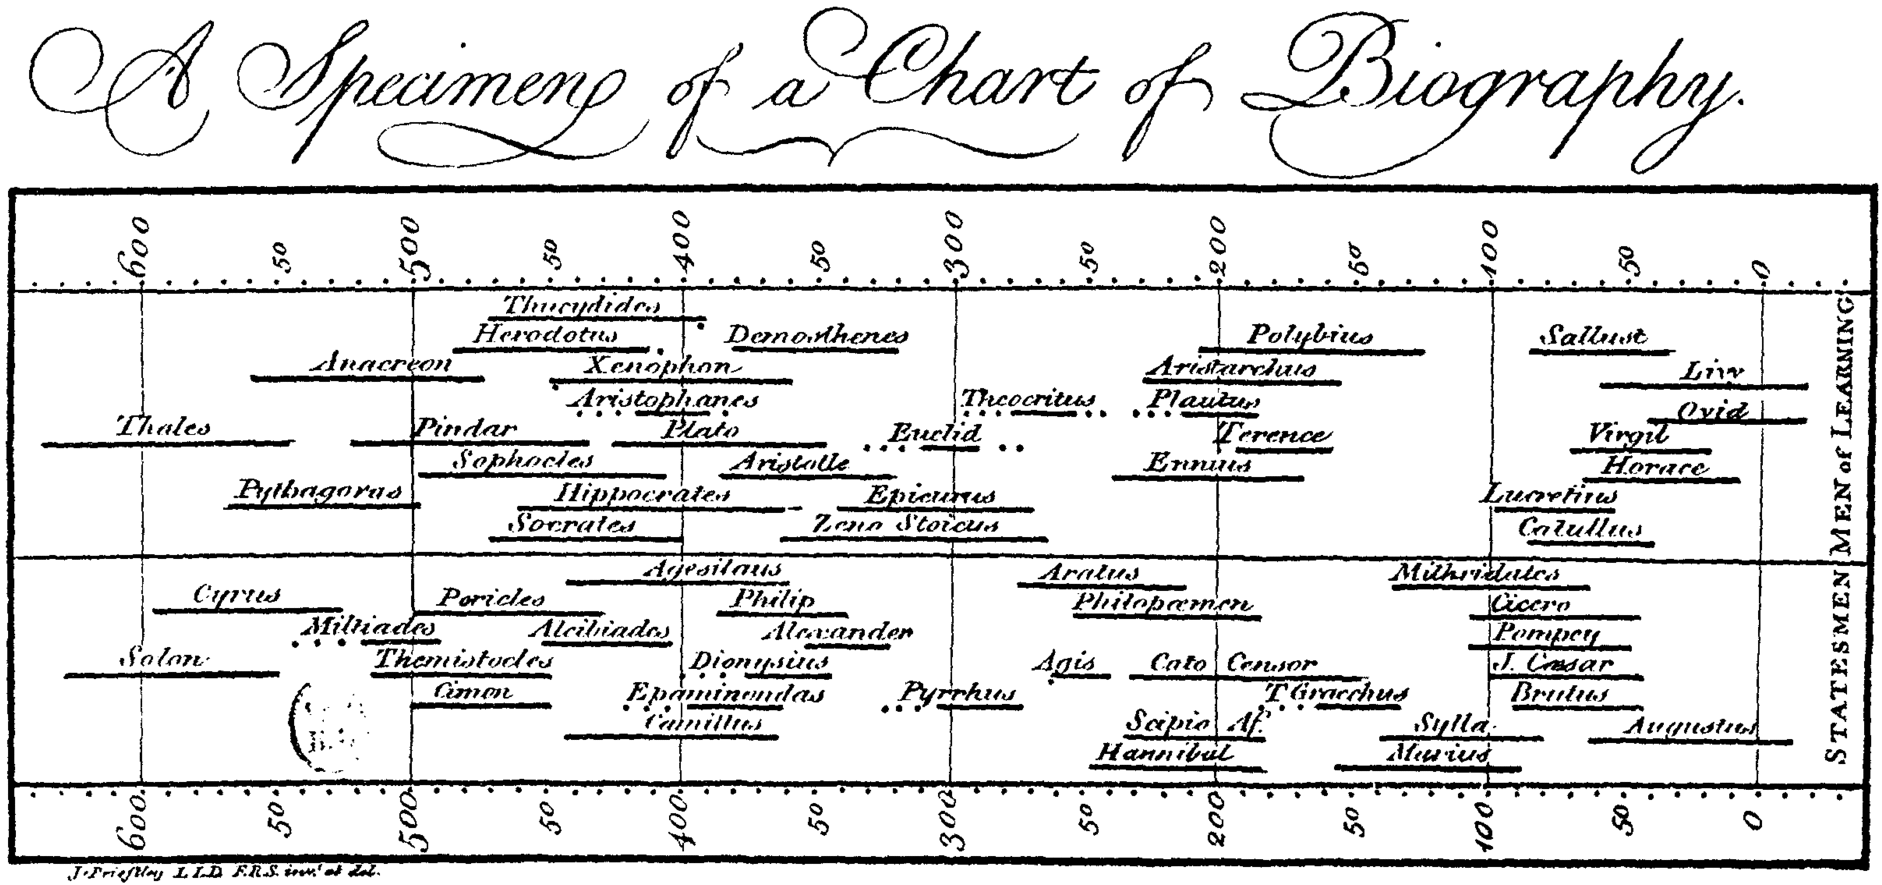
\includegraphics[width=0.9\textwidth]{c4.playfair.02.png}
  \end{figure}
\end{frame}

\begin{frame}
  \frametitle{统计图形 | 设计者 | 威廉·普莱费尔}
  \begin{figure}
    \centering
    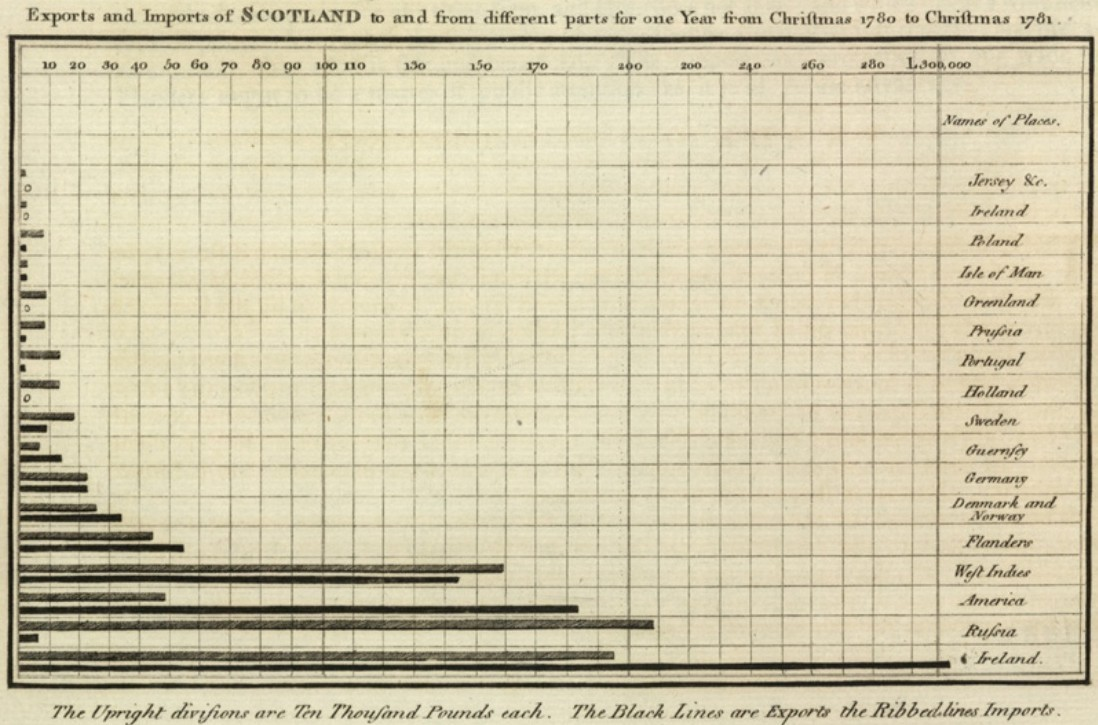
\includegraphics[width=0.9\textwidth]{c4.playfair.03.jpg}
  \end{figure}
\end{frame}

\begin{frame}
  \frametitle{统计图形 | 设计者 | 威廉·普莱费尔}
  \begin{figure}
    \centering
    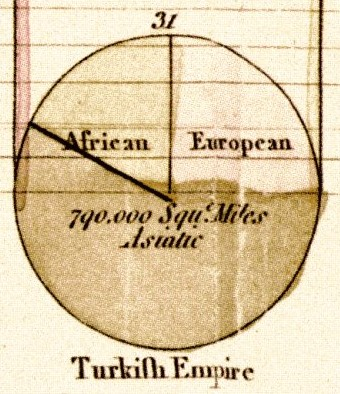
\includegraphics[width=0.45\textwidth]{c4.playfair.04.jpg}
    \caption{Pie chart from Playfair's Statistical Breviary (1801), showing the proportions of the Turkish Empire located in Asia, Europe and Africa before 1789.}
  \end{figure}
\end{frame}

\begin{frame}
  \frametitle{统计图形 | 设计者 | 南丁格尔}
  \begin{block}{南丁格尔}
    弗罗伦斯·南丁格尔,(Florence Nightingale),英国护士和统计学家。曾经运用统计图形来说服英国政府,以改善军队的卫生状况。\\
    \vspace{0.5em}
克里米亚战争时,她极力向英国军方争取在战地开设医院,为士兵提供医疗护理。她分析过堆积如山的军事档案,指出在克里米亚战役中,英军死亡的原因是在战场外感染疾病,及在战场上受伤后缺乏适当护理而伤重致死,真正死在战场上的人反而不多。她更用了圆形图以说明这些资料。\\
    \vspace{0.5em}
由于南丁格尔的贡献,让昔日地位低微的护士,社会地位与形象都大为提高,成为崇高的象征。“南丁格尔”也成为护士精神的代名词。
  \end{block}
\end{frame}

\begin{frame}
  \frametitle{统计图形 | 设计者 | 南丁格尔}
  \begin{block}{南丁格尔 vs. 统计}
南丁格尔从小就显示出对数学的天分,后来,南丁格尔成为视觉表现和统计图形的先驱。她所使用的圆饼图,虽然在1801年由威廉·普莱费尔所发明,但在当时仍是一个新颖的显示数据的方法。\\
\vspace{0.5em}
南丁格尔被描述为“在统计的图形显示方法上,是一个真正的先驱”, 她发展出极座标图饼图的形式(polar area diagram),或称为南丁格尔玫瑰图(Nightingale rose diagram),相当于现代圆形直方图(circular histogram),以说明在她管理的野战医院内,病人死亡率在不同季节的变化。她使用极座标图饼图,向不会阅读统计报告的国会议员,报告克里米亚战争的医疗条件。\\
\vspace{0.5em}
在1859年南丁格尔被选为英国皇家统计学会的第一个女成员,她后来成为美国统计协会的名誉会员。
  \end{block}
\end{frame}

\begin{frame}
  \frametitle{统计图形 | 设计者 | 南丁格尔}
  \begin{figure}
    \centering
    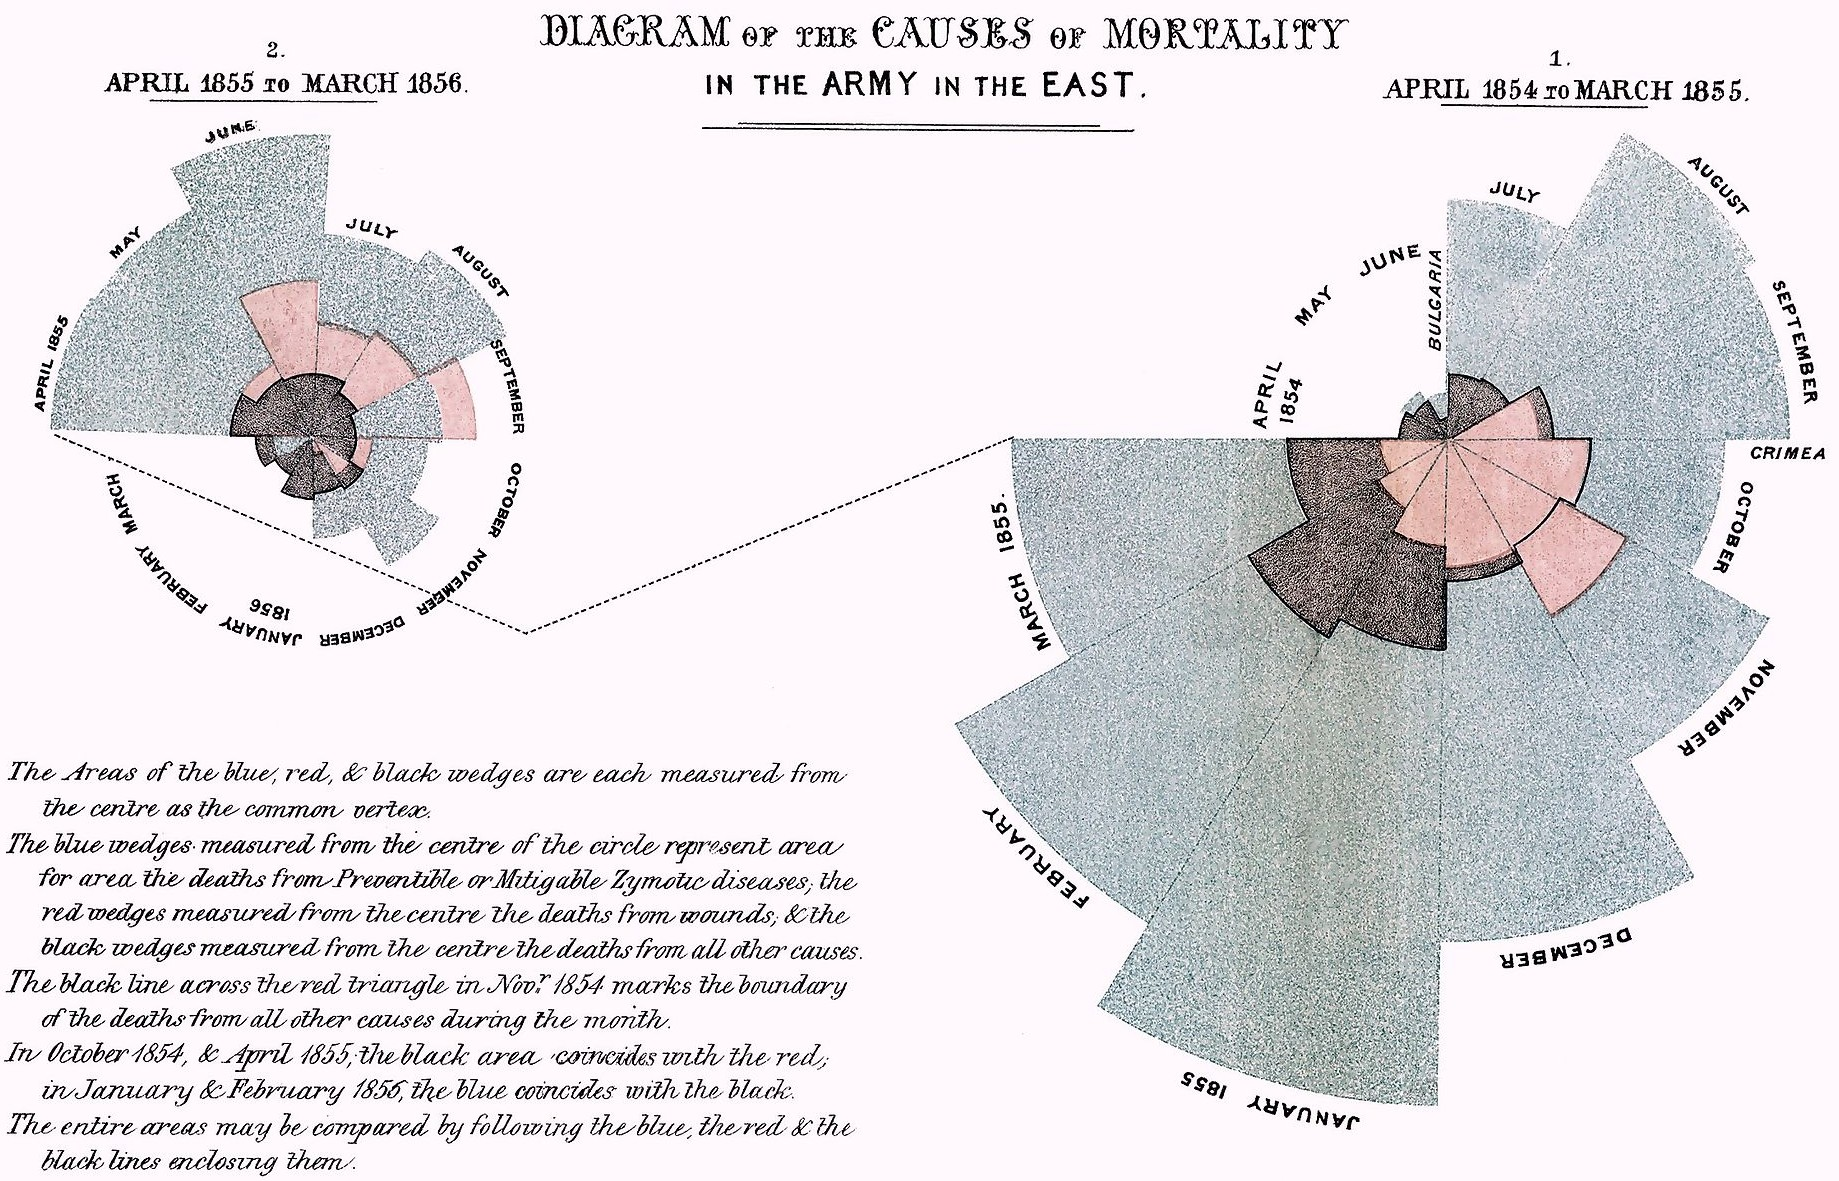
\includegraphics[width=0.9\textwidth]{c4.nightingale.01.jpg}
    \caption{弗罗伦斯·南丁格尔绘制的“东部军队死亡原因统计图”。}
  \end{figure}
\end{frame}

\begin{frame}
  \frametitle{统计图形 | 设计者 | 约翰·斯诺}
  \begin{block}{约翰·斯诺}
    绘制了1854伦敦霍乱死亡病例的分布图,从而发现了病源所在。斯诺的研究可以说是公共卫生学历史上一重大事件。\\
    \vspace{0.5em}
    约翰·斯诺(John Snow),英国内科医生,因在1854年宽街霍乱爆发事件研究中作出重大贡献,被认为是麻醉学和公共卫生医学的开拓者。\\
  \end{block}
\end{frame}

\begin{frame}
  \frametitle{统计图形 | 设计者 | 约翰·斯诺}
  \begin{figure}
    \centering
    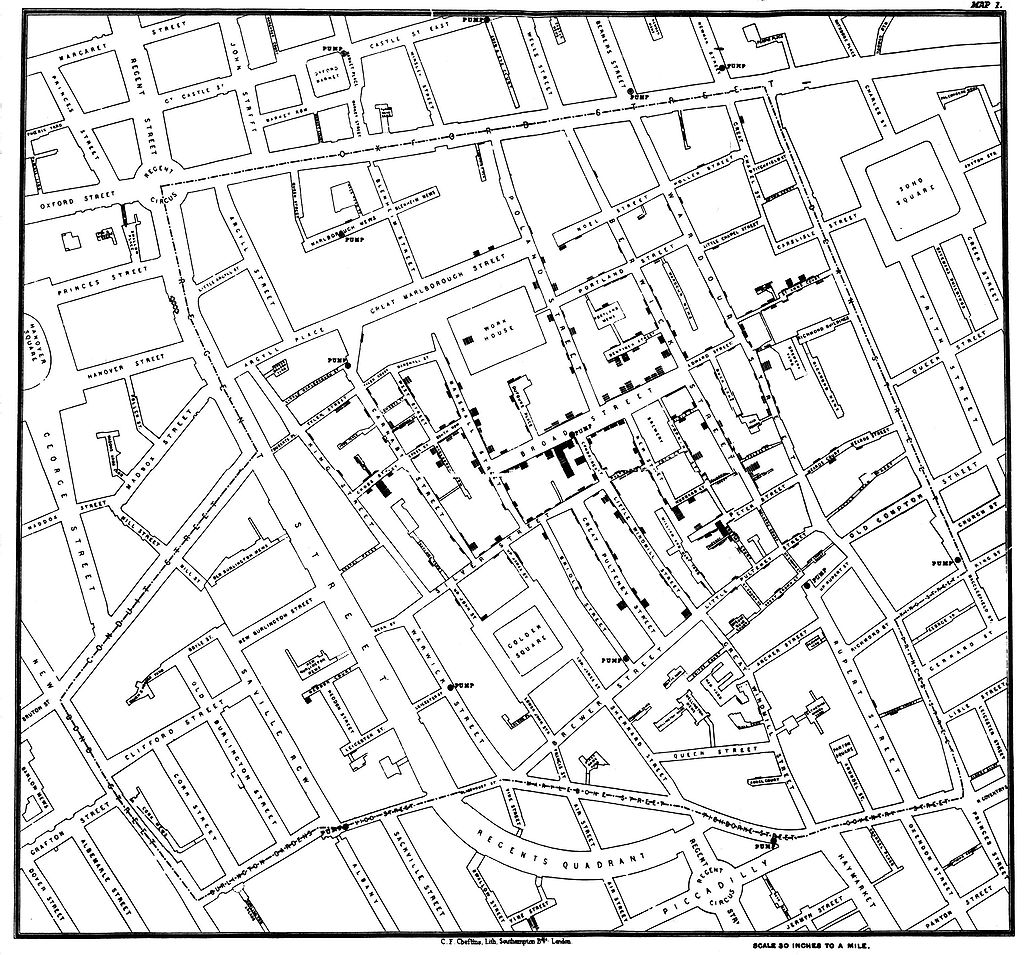
\includegraphics[width=0.7\textwidth]{c4.snow.01.jpg}
    \caption{1854年斯诺在伦敦霍乱爆发时研究个案时用的地图。}
  \end{figure}
\end{frame}

\begin{frame}
  \frametitle{统计图形 | 设计者 | 查尔斯·约瑟夫·密纳德}
  \begin{block}{查尔斯·约瑟夫·密纳德}
  设计了大量的地图;其中,最为著名的一幅描绘了拿破仑入侵俄国的活动。\\
  \vspace{0.5em}
  Charles Joseph Minard was a French civil engineer recognized for his significant contribution in the field of information graphics in civil engineering and statistics. Minard was, among other things, noted for his representation of numerical data on geographic maps.
  \end{block}
\end{frame}

\begin{frame}
  \frametitle{统计图形 | 设计者 | 查尔斯·约瑟夫·密纳德}
  \begin{figure}
    \centering
    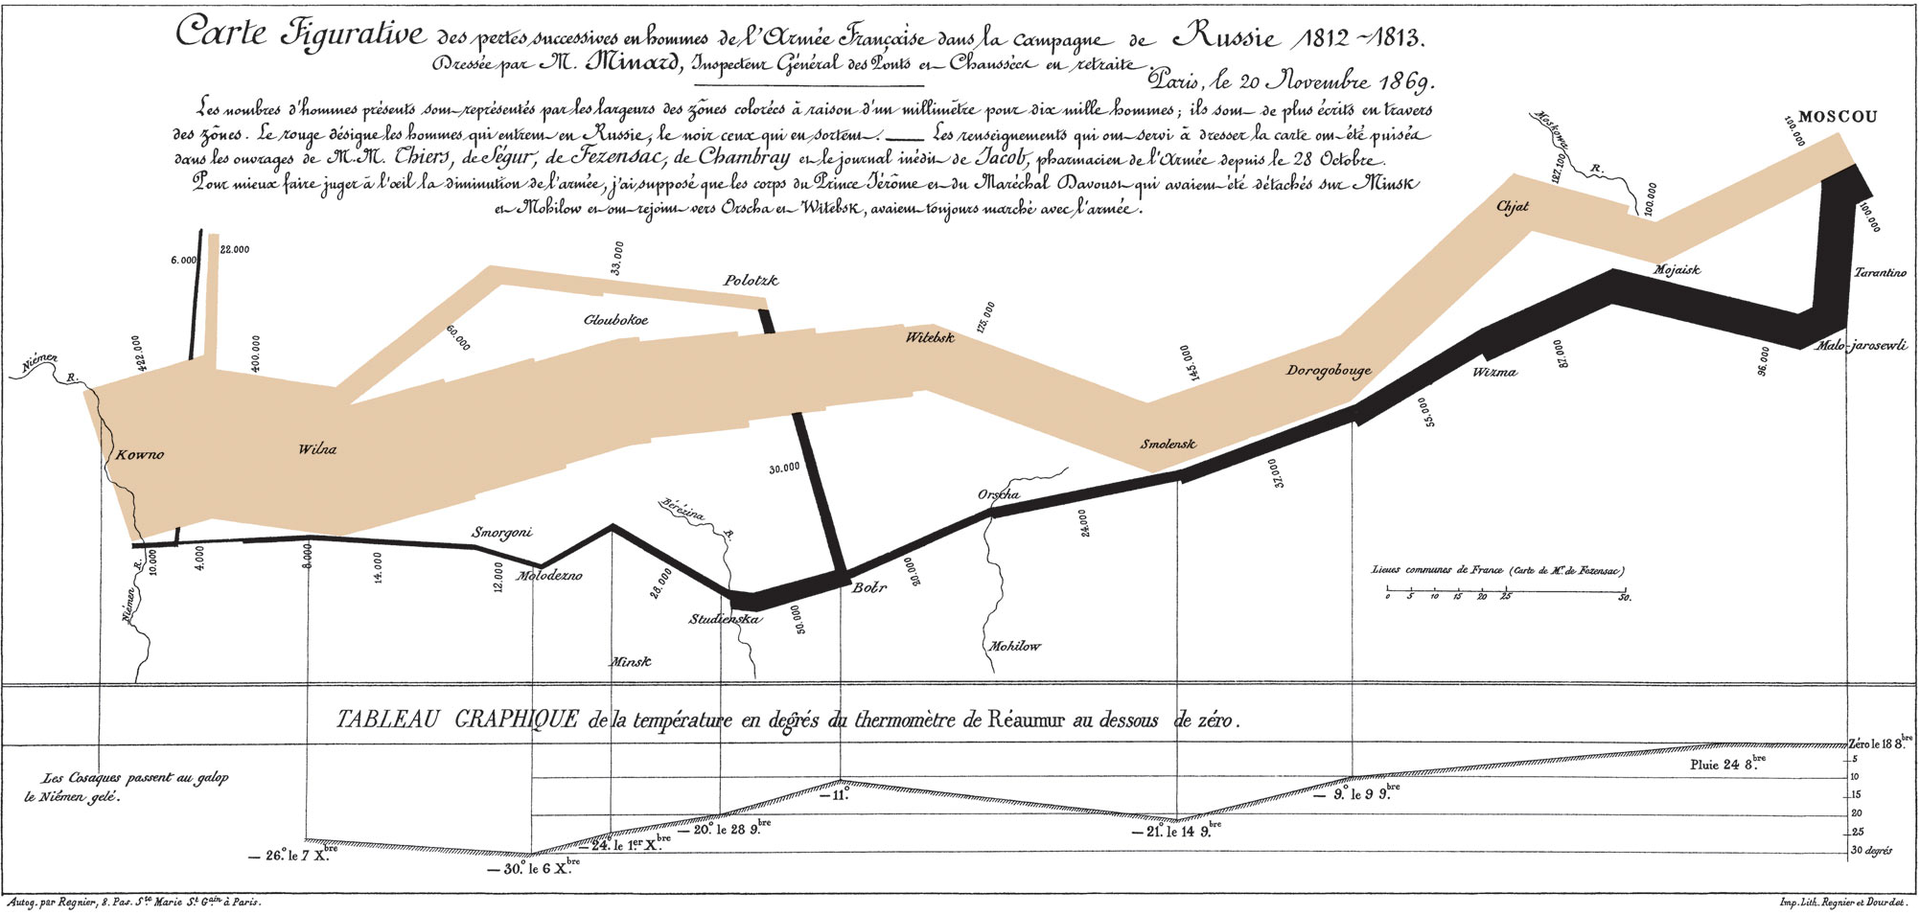
\includegraphics[width=\textwidth]{c4.minard.01.png}
    \caption{法国工程师查尔斯·约瑟夫·密纳德于1861年绘制的关于拿破仑入侵俄国的信息图形。}
  \end{figure}
\end{frame}

\begin{frame}
  \frametitle{统计图形 | 设计者 | 查尔斯·约瑟夫·密纳德}
  \begin{figure}
    \centering
    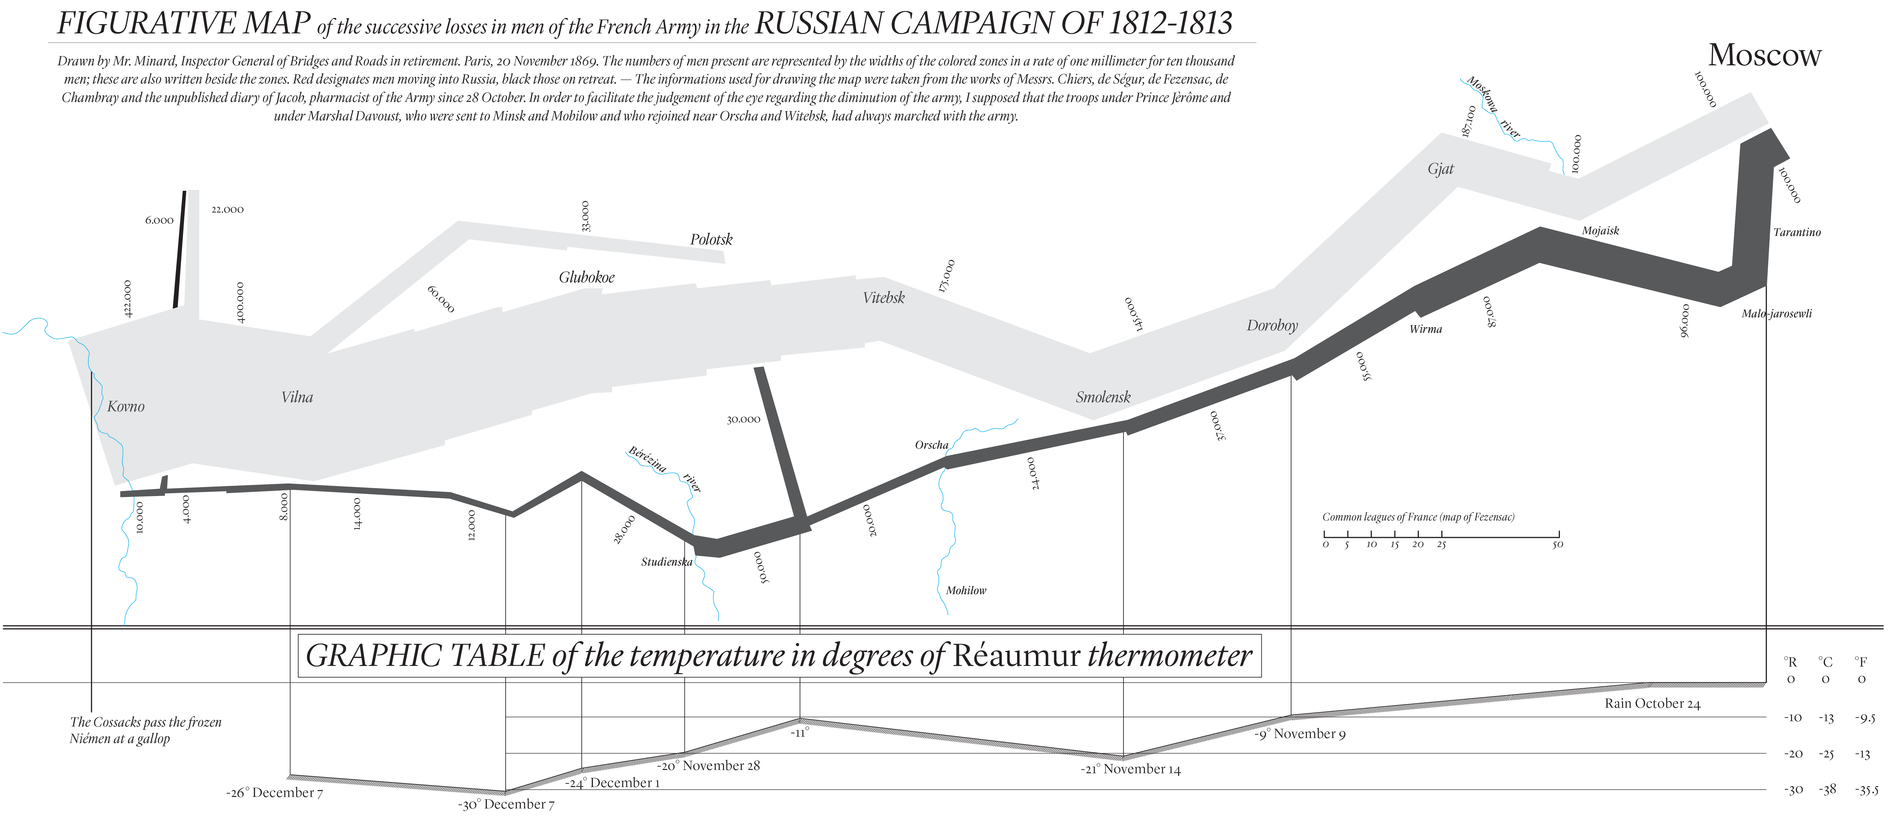
\includegraphics[width=\textwidth]{c4.minard.02.png}
  \end{figure}
\end{frame}

\begin{frame}
  \frametitle{统计图形 | 设计者 | 查尔斯·约瑟夫·密纳德}
  \begin{figure}
    \centering
    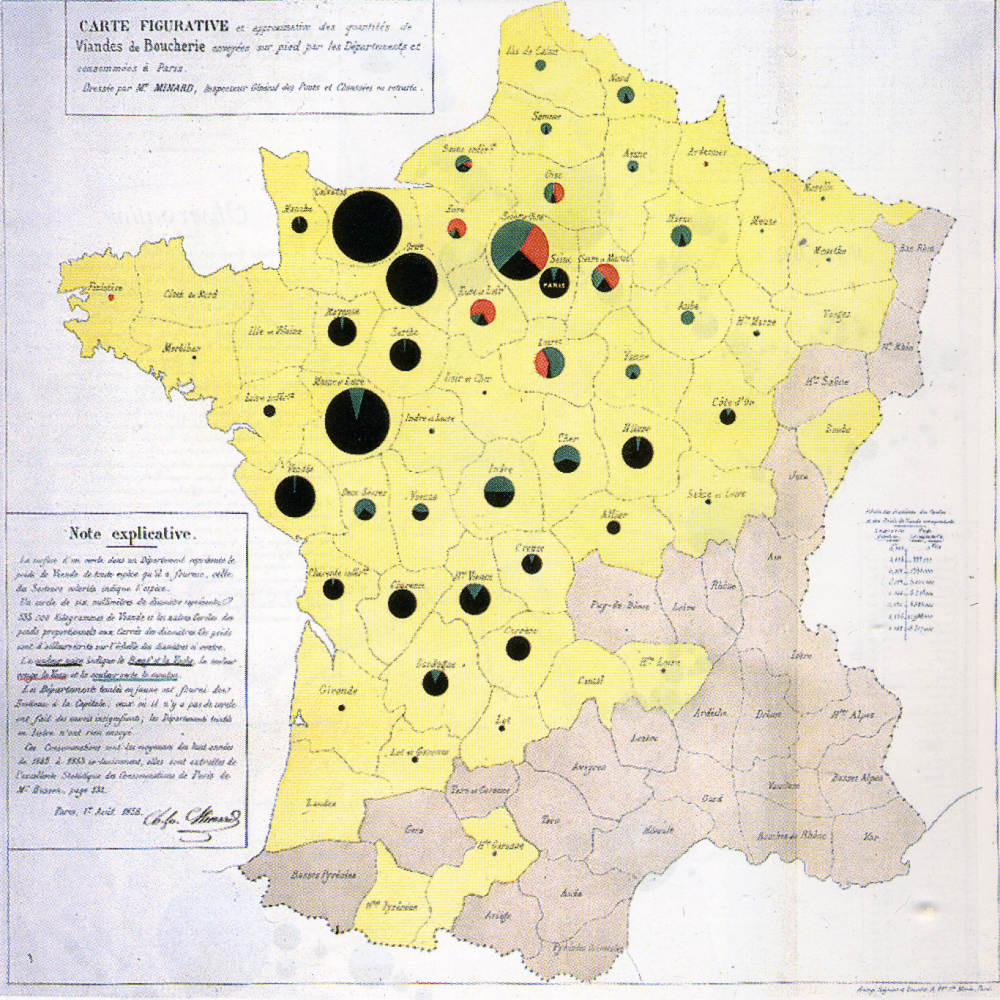
\includegraphics[width=0.55\textwidth]{c4.minard.03.png}
    \caption{Minard's map using pie charts to represent the cattle sent from all around France for consumption in Paris (1858).}
  \end{figure}
\end{frame}

\begin{frame}
  \frametitle{统计图形 | 设计者 | 奥图·纽拉特}
  \begin{block}{奥图·纽拉特}
    设计了一种特殊类型的统计图形,称为同型图(isotype)。这种图形工具的具体目的就是,通过对群众进行形象的可视化教育,来实现社会变革。\\
    \vspace{0.5em}
奥图·纽拉特(Otto Neurath),奥地利人,是个科学家、社会学家及经济学学者,在因纳粹而被迫逃离到英国前是维也纳学派的知名人物。    
  \end{block}
  \pause
  \begin{block}{同型图}
    Isotype图像符号,是奥图于1925年发表、经过系统化设计的图画文字。``ISOTYPE"(International System of Typographic Picture Education) 希望透过系统文的图像来取代文字,形成一种世界共通的语言,其本质类似于现在流行于网络的MSN/Emoji表情符号等。\\
    \vspace{0.5em}
    奥图曾试图用这种图画文字来取代沟通,虽然最后失败了,但是这种Isotype的概念,后来在ICON、标示等设计领域,有着十分深远的影响。
  \end{block}
\end{frame}

\begin{frame}
  \frametitle{统计图形 | 设计者 | 奥图·纽拉特}
  \begin{figure}
    \centering
    \includegraphics[width=0.8\textwidth]{c4.neurath.01.jpg}
    \caption{Pages from Neurath's International picture language, 1936.}
  \end{figure}
\end{frame}

\section{案例分析}
\subsection{操作纵轴}
\begin{frame}
  \frametitle{案例 | 纵轴 | 国民收入}
  \begin{block}{目标}
    用图形来显示国民收入怎样在一年内实现了10\%的增长。
  \end{block}
  \pause
  \begin{block}{绘图}
    \begin{enumerate}
      \item 在纸上用相互垂直的直线画出许多小方格。
      \item 在横轴的底部注明月份,在纵轴旁标上数字,单位是“十亿美元”。
      \item 在图中点出每个月的国民收入。
      \item 用直线将这些点连接起来。
    \end{enumerate}
  \end{block}
\end{frame}

\begin{frame}
  \frametitle{案例 | 纵轴 | 国民收入}
  \begin{figure}
    \centering
    \includegraphics[width=0.7\textwidth]{c4.case.line.income.01.png}
  \end{figure}
\end{frame}

\begin{frame}
  \frametitle{案例 | 纵轴 | 国民收入}
  \begin{block}{解析}
    \begin{itemize}
      \item 图清晰地显示了一年来的变化,而且变化是逐月反映出来的。
      \item 能看出上涨趋势,但却并不振奋人心。
      \item 传递信息的目的达到了,但缺乏渲染的效果(用于辩论、推销、推动……)。
    \end{itemize}
  \end{block}
  \pause
  \begin{block}{原因}
    \begin{itemize}
      \item 纵轴从原点即“0”开始
      \item 整张图形是按比例绘制的
    \end{itemize}
  \end{block}
\end{frame}

\begin{frame}
  \frametitle{案例 | 纵轴 | 国民收入}
  \begin{block}{抹去图形的底部}
    数据是相同的,所以图形也相同,除了图形给人留下的印象不同之外,没有进行任何的伪造。
  \end{block}
  \vspace{-0.5em}
  \begin{figure}
    \centering
    \includegraphics[width=0.9\textwidth]{c4.case.line.income.02.png}
  \end{figure}
  \pause
  \vspace{-0.5em}
  \begin{block}{解析}
    眼睛不能“理解”被抹去的部分,这才导致微小的上升最终变成了惊人的增长。
  \end{block}
\end{frame}

\begin{frame}
  \frametitle{案例 | 纵轴 | 国民收入}
  \begin{block}{改变横坐标与纵坐标的比例关系}
    将纵坐标的每一个刻度缩减为原来的1/10即可,没有人规定不能这么做,而这将会产生一张更加完美的图形——使朴实的10\%的增长率看上去比100\%的增长率更让人振奋。
  \end{block}
  \vspace{-0.5em}
  \begin{figure}
    \centering
    \includegraphics[width=0.5\textwidth]{c4.case.line.income.03.png}
  \end{figure}
\end{frame}

\begin{frame}
  \frametitle{案例 | 纵轴 | 国民收入}
  \begin{block}{令人惊奇的图形}
    \begin{itemize}
      \item 任何看到这幅图的人都会强烈地感觉到在国家的各条经济命脉上正快速地积累着大量的财富。
      \item 这相当于将“国民收入增长了10个百分点”改写成了“国民收入惊人地攀升了10个百分点”。
      \item 显然图形比文字更有效,因为图形中不存在任何形容词和副词来破坏它所具有的客观性幻觉,而且谁也无法指责你。
    \end{itemize}
  \end{block}
\end{frame}

\begin{frame}
  \frametitle{案例 | 纵轴 | 新闻发言人对企业经营业绩的操作}
  \begin{block}{“灰姑娘”到“白雪公主”的蜕变}
    \begin{figure}
      \centering
      \visible<1->{\includegraphics[width=0.22\textwidth]{c4.case.line.company.01.png}}
      \visible<2->{\includegraphics[width=0.28\textwidth]{c4.case.line.company.02.png}}
      \visible<3->{\includegraphics[width=0.22\textwidth]{c4.case.line.company.03.png}}
      \visible<4->{\includegraphics[width=0.155\textwidth]{c4.case.line.company.04.png}}
    \end{figure}
  \end{block}
\end{frame}

\begin{frame}
  \frametitle{案例 | 纵轴 | 政府支出}
  \begin{figure}
    \centering
    \includegraphics[width=0.58\textwidth]{c4.case.line.out.01.png}
  \end{figure}
  \vspace{-1em}
  \begin{block}{vs.}
    \begin{itemize}
      \item 保持稳定:折线客观地反映了4\%的增长率
      \item 急剧上升:折线从底部激增到顶端,将原本仅仅4\%的增长率描绘的仿佛是400\%
    \end{itemize}
  \end{block}
\end{frame}

\begin{frame}
  \frametitle{案例 | 纵轴 | 标致汽车的广告}
  \begin{figure}
    \centering
    \includegraphics[width=0.48\textwidth]{c4.case.line.car.01.png}\quad
    \includegraphics[width=0.43\textwidth]{c4.case.line.car.02.png}
  \end{figure}
\end{frame}

\begin{frame}
  \frametitle{案例 | 纵轴 | 美国道琼斯股票指数}
  \begin{block}{非凡的牛市!?}
    \begin{figure}
      \centering
      \includegraphics[width=0.7\textwidth]{c4.case.line.shock.01.png}
    \end{figure}
  \end{block}
\end{frame}

\begin{frame}
  \frametitle{案例 | 纵轴 | 妇女和犯罪}
  \begin{block}{妇女更加倾向于使用暴力?}
    \begin{figure}
      \centering
      \includegraphics[width=0.68\textwidth]{c4.case.line.woman.01.png}
    \end{figure}
    \vspace{-1em}
    \pause
    从300000人上升到335000人,标志着4年内上升了11.7\%。或者说,平均每年的犯罪增长率不到3\%。\\
    \vspace{0.2em}
如果不是从300000开始,而是从零开始,那么,事实立即就会很清楚:女性违法犯罪行为的上升速度并不是非同寻常,相反还落后于一般刑事犯罪的上升幅度。也就是说,与男人相比,妇女并不容易表现得暴怒与粗暴,而是表现出平和与友好。
  \end{block}
\end{frame}

\begin{frame}
  \frametitle{案例 | 纵轴 | 柱状图}
  \begin{block}{一个被截短的柱状图与被截短的折线图实乃一丘之貉}
  \begin{figure}
    \centering
    \includegraphics[width=0.9\textwidth]{c4.case.line.bar.01.png}
  \end{figure}
  \end{block}
\end{frame}

\begin{frame}
  \frametitle{案例 | 纵轴 | 德意志银行的顾客发展演变过程}
  \begin{figure}
    \centering
    \includegraphics[width=0.5\textwidth]{c4.case.line.bank.01.png}\quad
    \includegraphics[width=0.46\textwidth]{c4.case.line.bank.02.png}
  \end{figure}
\end{frame}

\subsection{操作横轴}
\begin{frame}
  \frametitle{案例 | 横轴 | 延伸横坐标}
  \begin{block}{对坐标的一部分进行延伸或者收缩}
    \begin{itemize}
      \item<1-> 在直线中,绝对增长在所有阶段都是一样的。
      \item<2-> 为了从感觉上来弱化这种增长趋势,人们一般会把横坐标画得更长一些。
      \item<3-> 如果为了从感觉上来强化这种增长,人们一般会从希望的时间点处开始把横坐标画得更短一些。
    \end{itemize}
    \begin{figure}
      \centering
      \visible<1->{\includegraphics[width=0.3\textwidth]{c4.case.line.axis.01.png}}
      \visible<2->{\includegraphics[width=0.33\textwidth]{c4.case.line.axis.02.png}}
      \visible<3->{\includegraphics[width=0.33\textwidth]{c4.case.line.axis.03.png}}
    \end{figure}
  \end{block}
\end{frame}

\begin{frame}
  \frametitle{案例 | 横轴 | 英国汽车工业}
  \begin{block}{1972~1988年发展的上升与下滑历程}
    \begin{figure}
      \centering
      \includegraphics[width=0.8\textwidth]{c4.case.line.car.03.png}
    \end{figure}
  \end{block}
\end{frame}

\begin{frame}
  \frametitle{案例 | 横轴 | 联邦德国的邮政资费}
  \begin{block}{邮资持续不变的假象}
    \begin{figure}
      \centering
      \includegraphics[width=0.8\textwidth]{c4.case.line.stamp.01.png}
    \end{figure}
  \end{block}
\end{frame}

\subsection{增减信息}
\begin{frame}
  \frametitle{案例 | 信息 | 自我宣传}
  \begin{block}{广告代理机构宣传自己的广告}
    \begin{figure}
      \centering
      \includegraphics[width=0.9\textwidth]{c4.case.line.other.01.png}
    \end{figure}
  \end{block}
\end{frame}

\begin{frame}
  \frametitle{案例 | 信息 | 自我宣传}
  \begin{block}{广告代理机构宣传自己的广告}
图中曲线意欲向人们显示这家广告公司年复一年惊人的发展趋势。但途中没有一个数字,这样一来,它既可以代表一个骇人的发展速度,每年翻番或增长几百万美金,又可以意味着在年十亿总收入的基础上,增加了一美元或两美元相对稳定的蛇状爬行。但仅从图上看,其发展速度让人印象深刻。
  \end{block}
\end{frame}

\begin{frame}
  \frametitle{案例 | 信息 | 薄饼}
  \begin{block}{薄饼“在2分钟之内开始提供能量”}
    \begin{figure}
      \centering
      \includegraphics[width=0.8\textwidth]{c4.case.line.other.02.png}
    \end{figure}
  \end{block}
\end{frame}

\begin{frame}
  \frametitle{案例 | 信息 | 经济上升}
  \begin{block}{经济上升}
  \begin{figure}
    \centering
    \includegraphics[width=0.9\textwidth]{c4.case.line.other.06.png}
  \end{figure}
  \end{block}
\end{frame}

\begin{frame}
  \frametitle{案例 | 信息 | “马屁精”}
  \begin{block}{使用相同的数据同时取悦共和党和民主党}
    \begin{figure}
      \centering
      \includegraphics[width=0.51\textwidth]{c4.case.line.other.04.png}\quad
      \includegraphics[width=0.42\textwidth]{c4.case.line.other.05.png}
    \end{figure}
  \end{block}
\end{frame}

\begin{frame}
  \frametitle{案例 | 信息 | 德国纺织工业}
  \begin{block}{德国纺织工业去向何方}
    \begin{figure}
      \centering
      \includegraphics[width=0.9\textwidth]{c4.case.line.other.07.png}
    \end{figure}
  \end{block}
\end{frame}

\begin{frame}
  \frametitle{案例 | 信息 | 美国制造业}
  \begin{block}{美国制造业的完整故事}
    \begin{figure}
      \centering
      \includegraphics[width=0.9\textwidth]{c4.case.line.other.03.png}
    \end{figure}
  \end{block}
\end{frame}

\begin{frame}
  \frametitle{案例 | 信息 | 广播电台的市场份额}
  \begin{block}{双雄争霸 vs. 三足鼎立}
    \begin{figure}
      \centering
      \includegraphics[width=0.7\textwidth]{c4.case.line.radio.01.png}
    \end{figure}
    \vspace{-1em}
    \pause
两个受欢迎的广播电台的实际情况是,每个广播电台都只拥有7\%的广播听众,而第三位的广播电台和其他广播电台拥有4\%的广播听众。换句话说,对于在广播电台做广告来说,每个广播电台都是一样的,没有一个广播电台能够控制并独占市场,受众最多的两个广播电台与其他广播电台之间的“巨大的”差距仅仅是一个幻象而已。
  \end{block}
\end{frame}

\subsection{趋势外推}
\begin{frame}
  \frametitle{案例 | 趋势 | 德国股份公司的收益}
  \begin{block}{一个过去的趋势在未来的10年得到了进一步的延续与升级}
    \begin{figure}
      \centering
      \includegraphics[width=0.6\textwidth]{c4.case.line.ten.01.png}
    \end{figure}
  \end{block}
\end{frame}

\begin{frame}
  \frametitle{案例 | 趋势 | 黄金价格}
  \begin{block}{黄金价格的未来趋势}
    \begin{figure}
      \centering
      \includegraphics[width=0.6\textwidth]{c4.case.line.gold.01.png}
    \end{figure}
  \end{block}
\end{frame}

\begin{frame}
  \frametitle{案例 | 趋势 | 股指的走势}
  \begin{figure}
    \centering
    \includegraphics[width=0.43\textwidth]{c4.case.line.shock.02.png}\quad
    \includegraphics[width=0.52\textwidth]{c4.case.line.shock.03.png}
  \end{figure}
\end{frame}

\begin{frame}
  \frametitle{案例 | 趋势 | 艾滋病未来的发展趋势}
  \begin{figure}
    \centering
    \includegraphics[width=0.9\textwidth]{c4.case.line.hiv.01.png}
  \end{figure}
\end{frame}

\begin{frame}
  \frametitle{案例 | 趋势 | “罗马俱乐部”的末日论}
  \begin{block}{农田需求}
    \begin{figure}
      \centering
      \includegraphics[width=0.7\textwidth]{c4.case.line.land.01.png}
    \end{figure}
  \end{block}
\end{frame}

\begin{frame}
  \frametitle{案例 | 趋势 | “罗马俱乐部”的末日论}
  \begin{block}{大气环境中的二氧化碳}
    \begin{figure}
      \centering
      \includegraphics[width=0.48\textwidth]{c4.case.line.air.01.png}
    \end{figure}
  \end{block}
\end{frame}

\subsection{一维图形}
\begin{frame}
  \frametitle{案例 | 维度 | 引言}
  \begin{block}{形象图形}
    形象图形,又称为象形图,它的前身是普通的柱状图,在比较两种或两种以上事物某个方面的具体数量时,柱状图是一种便捷常用的方法。\\
但是柱状图也具有欺骗性:在描述单一物体时,柱体改变宽度的同时,长度也发生变化;在描述三维物体时,物体的体积又不容易进行比较,以上任何一种情况都提醒我们应该对柱状图保留一些怀疑。\\
  \end{block}
  \pause
  \begin{block}{双刃剑}
    \begin{itemize}
      \item 用一个小人来表示成千上万的人,一个钱袋或一堆硬币表示一千英镑或者百万美金,一篇牛肉表示明年牛肉的供应量,这些都是形象的图形表示。
      \item 由于这种图形非常吸引眼球,所以可以作为一种有用的工具,但同时它也能摇身一变,成为一个老练、狡猾而且成功的骗子。
    \end{itemize}
  \end{block}
\end{frame}

\begin{frame}
  \frametitle{案例 | 维度 | 工资}
  \begin{block}{目标}
    \begin{itemize}
      \item 比较两个数据——英国与罗坦提亚某工种公认的平均周工资,假设数值分别为30英镑和15英镑。
      \item 未说出的目的——说明英国工人比罗坦提亚工人的境况好得多(差距渲染得越大论据越充分)。
      \item 同时避免麻烦——希望你能从中推断出什么,或者留下一个夸张的印象,而作者又不会因此惹上麻烦。
    \end{itemize}
  \end{block}
  \pause
  \begin{block}{方法}
    \begin{itemize}
      \item 直接将数字打印出来
      \item 为了吸引注意,画出柱状图
    \end{itemize}
  \end{block}
\end{frame}

\begin{frame}
  \frametitle{案例 | 维度 | 工资}
  \begin{figure}
    \centering
    \includegraphics[width=0.9\textwidth]{c4.case.1d.bar.01.png}
  \end{figure}
  \vspace{-1em}
  \begin{block}{解析}
    \begin{itemize}
      \item 清楚且忠于事实的图形——收入是1:2的比例关系,图中两根柱体的比例也是1:2。
      \item 图形并不吸引眼球!——用钱袋来表示收入。
    \end{itemize}
  \end{block}
\end{frame}

\begin{frame}
  \frametitle{案例 | 维度 | 工资}
  \begin{block}{钱袋图}
    画一个钱袋用来表示罗坦提亚人的15英镑,然后再画一个高两倍的钱袋代表英国佬的30英镑。还是1:2的比例……对吗?
  \end{block}
  \vspace{-0.5em}
  \begin{figure}
    \centering
    \includegraphics[width=0.75\textwidth]{c4.case.1d.bag.01.png}
  \end{figure}
\end{frame}

\begin{frame}
  \frametitle{案例 | 维度 | 工资}
  \begin{block}{解析}
    \begin{itemize}
      \item 直观的感受——英国佬的收入使得罗坦提亚工人相形见绌。
      \item 奥妙的关键——既然第二个袋子比第一个高一倍,也应该同样宽一倍,那么占用纸张的空间就不是2倍而变成4倍。
      \item 数字全是2:1,但视觉效果却是4:1,而在大多数时候视觉效果起着决定性的作用。
      \item 实际事物往往是三维的——如果一个钱袋里有15英镑,另一个钱袋里面就不仅仅只装了30英镑,而应该是120英镑(15英镑的8倍)!
      \item 明明说的是“2倍”,却最终让你留下了令人震惊的8倍的印象。
    \end{itemize}
  \end{block}
\end{frame}

\begin{frame}
  \frametitle{案例 | 维度 | 收入}
  \begin{figure}
    \centering
    \visible<1->{\includegraphics[width=0.23\textwidth]{c4.case.1d.income.01.png}}
    \visible<2->{\includegraphics[width=0.38\textwidth]{c4.case.1d.income.02.png}}
    \visible<3->{\includegraphics[width=0.35\textwidth]{c4.case.1d.income.03.png}}
  \end{figure}
\end{frame}

\begin{frame}
  \frametitle{案例 | 维度 | 住房面积}
  \begin{block}{联邦德国新州和老州的住房面积}
    \begin{figure}
      \centering
      \includegraphics[width=0.9\textwidth]{c4.case.1d.house.01.png}
    \end{figure}
    \vspace{-0.5em}
    不用住房的面积而是用住房的边长来表示,因此,两个平面图的面积就是82:58,而是像实际生活中那样为116:58(住房面积不是多了41\%,而是多了100\%)。
  \end{block}
\end{frame}

\begin{frame}
  \frametitle{案例 | 维度 | 汽车销售数量}
  \begin{figure}
    \centering
    \includegraphics[width=0.7\textwidth]{c4.case.1d.car.01.png}
  \end{figure}
\end{frame}

\begin{frame}
  \frametitle{案例 | 维度 | 二氧化碳排放量}
  \begin{figure}
    \centering
    \includegraphics[width=0.43\textwidth]{c4.case.1d.co2.01.png}
  \end{figure}
\end{frame}

\begin{frame}
  \frametitle{案例 | 维度 | 欧盟国中每个就业者的补贴状况}
  \begin{figure}
    \centering
    \includegraphics[width=0.9\textwidth]{c4.case.1d.om.01.png}
  \end{figure}
\end{frame}

\begin{frame}
  \frametitle{案例 | 维度 | 药品消费}
  \begin{figure}
    \centering
    \includegraphics[width=0.45\textwidth]{c4.case.1d.drug.01.png}
  \end{figure}
\end{frame}

\begin{frame}
  \frametitle{案例 | 维度 | 垃圾量}
  \begin{figure}
    \centering
    \includegraphics[width=0.9\textwidth]{c4.case.1d.trash.01.png}
  \end{figure}
\end{frame}

\begin{frame}
  \frametitle{案例 | 维度 | 包装费用}
  \begin{figure}
    \centering
    \includegraphics[width=0.4\textwidth]{c4.case.1d.box.01.png}
  \end{figure}
\end{frame}

\begin{frame}
  \frametitle{案例 | 维度 | 钢产量}
  \begin{block}{目的}
    美国钢铁协会希望通过图形显示20年来钢铁产量有了大幅度的提高,说明该行业表现出色,从而指出政府的任何干预都是不必要的。
  \end{block}
  \vspace{-0.5em}
  \begin{figure}
    \centering
    \includegraphics[width=0.6\textwidth]{c4.case.1d.iron.01.png}
  \end{figure}
\end{frame}

\begin{frame}
  \frametitle{案例 | 维度 | 钢产量}
  \begin{block}{解析——变成魔术的算术}
    \begin{itemize}
      \item 表示前10年增产1000万吨的鼓风炉,其高度仅是表示后10年增产1425万吨鼓风炉高度的2/3。但是眼睛看到的两个鼓风炉,一个却是另一个的3倍。嘴上说的是1.5倍,看起来却是3倍。
      \item 从水平上看,第二个鼓风炉似乎“胖些”,其宽度与其邻居的比例失调。
      \item 鼓风炉内的黑色条块,代表这熔化的铁,其长度看上去是10年前的2.5倍。于是,50\%的增长率被画成了150\%的增长率,视觉效果又将其变成1500\%的增长率。
    \end{itemize}
  \end{block}
\end{frame}

\begin{frame}
  \frametitle{案例 | 维度 | 奶牛}
  \begin{figure}
    \centering
    \includegraphics[width=0.8\textwidth]{c4.case.1d.nn.01.png}
  \end{figure}
  \vspace{-1em}
  \pause \pause \pause \pause
  \begin{block}{效果}
    \begin{itemize}
      \item 真实目的:1860年美国只有800万头奶牛,而一个世纪后该数量超过了2500万头。
      \item 实际效果:现在的牛要比以前的牛大得多。
    \end{itemize}
  \end{block}
\end{frame}

\begin{frame}
  \frametitle{案例 | 维度 | 犀牛}
  \begin{figure}
    \centering
    \includegraphics[width=0.55\textwidth]{c4.case.1d.xn.01.png}
  \end{figure}
\end{frame}

\subsection{地理地图}
\begin{frame}
  \frametitle{案例 | 地图 | 世界的中心}
  \begin{block}{哪里是世界的中心?}
    \begin{figure}
      \centering
      \includegraphics[width=0.5\textwidth]{c4.case.world.01.png}\quad
      \includegraphics[width=0.43\textwidth]{c4.case.world.02.png}
    \end{figure}
  \end{block}
\end{frame}

\begin{frame}
  \frametitle{案例 | 地图 | 人口密度图}
  \begin{block}{联邦德国的居民密度}
    \begin{figure}
      \centering
      \includegraphics[width=0.7\textwidth]{c4.case.population.01.png}
    \end{figure}
  \end{block}
\end{frame}

\begin{frame}
  \frametitle{案例 | 地图 | 医生职位}
  \begin{block}{“空的”医生职位}
    \begin{figure}
      \centering
      \includegraphics[width=0.75\textwidth]{c4.case.doctor.01.png}
    \end{figure}
  \end{block}
\end{frame}

\section{知识拓展}
\subsection{埃舍尔}
\begin{frame}
  \frametitle{埃舍尔 | 作品}
  \begin{figure}
    \centering
    \includegraphics[width=0.45\textwidth]{c4.escher.05.jpg}\quad
    \includegraphics[width=0.47\textwidth]{c4.escher.30.jpg}
  \end{figure}
\end{frame}

\begin{frame}
  \frametitle{埃舍尔 | 作品}
  \begin{figure}
    \centering
    \includegraphics[width=0.49\textwidth]{c4.escher.07.jpg}\quad
    \includegraphics[width=0.47\textwidth]{c4.escher.08.jpg}
  \end{figure}
\end{frame}

\begin{frame}
  \frametitle{埃舍尔 | 作品}
  \begin{figure}
    \centering
    \includegraphics[width=0.58\textwidth]{c4.escher.32.jpg}\quad
    \includegraphics[width=0.37\textwidth]{c4.escher.36.jpg}
  \end{figure}
\end{frame}

\begin{frame}
  \frametitle{埃舍尔 | 作品}
  \begin{figure}
    \centering
    \includegraphics[width=0.54\textwidth]{c4.escher.31.jpg}\quad
    \includegraphics[width=0.42\textwidth]{c4.escher.34.jpg}
  \end{figure}
\end{frame}

\begin{frame}
  \frametitle{埃舍尔 | 作品}
  \begin{figure}
    \centering
    \includegraphics[width=0.39\textwidth]{c4.escher.20.jpg}\quad
    \includegraphics[width=0.53\textwidth]{c4.escher.21.jpg}
  \end{figure}
\end{frame}

\begin{frame}
  \frametitle{埃舍尔 | 作品}
  \begin{figure}
    \centering
    \includegraphics[width=0.39\textwidth]{c4.escher.01.jpg}\quad
    \includegraphics[width=0.56\textwidth]{c4.escher.02.jpg}
  \end{figure}
\end{frame}

\begin{frame}
  \frametitle{不可能的图形}
  \begin{columns}
    \column{0.45\textwidth}
    \begin{block}{魔鬼叉子}
      \begin{figure}
        \centering
        \includegraphics[width=0.9\textwidth]{c4.escher.40.png}
      \end{figure}
    \end{block}
    \column{0.5\textwidth}
    \begin{block}{彭罗斯阶梯}
      \begin{figure}
        \centering
        \includegraphics[width=0.9\textwidth]{c4.escher.41.png}
      \end{figure}
    \end{block}
  \end{columns}
\end{frame}

\begin{frame}
  \frametitle{不可能的图形}
  \begin{columns}
    \column{0.43\textwidth}
    \begin{block}{不可能的方块}
      \begin{figure}
        \centering
        \includegraphics[width=0.93\textwidth]{c4.escher.39.png}
      \end{figure}
    \end{block}
    \column{0.5\textwidth}
    \begin{block}{潘洛斯三角}
      \begin{figure}
        \centering
        \includegraphics[width=0.9\textwidth]{c4.escher.24.png}
      \end{figure}
    \end{block}
  \end{columns}
\end{frame}

\begin{frame}
  \frametitle{其他}
  \begin{columns}
    \column{0.3\textwidth}
    \begin{block}{莫比乌斯带}
      \begin{figure}
        \centering
        \includegraphics[width=0.9\textwidth]{c4.escher.22.jpg}
      \end{figure}
    \end{block}
    \column{0.3\textwidth}
    \begin{block}{克莱因瓶}
      \begin{figure}
        \centering
        \includegraphics[width=0.93\textwidth]{c4.escher.23.png}
      \end{figure}
    \end{block}
  \end{columns}
\end{frame}

\begin{frame}
  \frametitle{不可能的图片}
  \begin{block}{不可能的图片}
    \begin{itemize}
      \item \href{http://news.xinhuanet.com/tech/2009-03/25/content_11072865.htm}{有趣的“不可能图形”:眼睛欺骗了你}
      \item \href{http://www.360doc.com/content/14/0626/17/699582_390050495.shtml}{不可能图片}
      \item \href{http://www.yi2.net/article/201606/13115.html}{不可能图形,眼见不一定为实}
      \item \href{http://yaoyao33.lofter.com/post/bcfa4_70ac2d3}{不可思议的幻觉图}
      \item \href{https://cn.depositphotos.com/vector-images/\%E4\%B8\%8D\%E5\%8F\%AF\%E8\%83\%BD\%E7\%9A\%84\%E7\%89\%A9\%E4\%BD\%93.html}{不可能的物体}
    \end{itemize}
  \end{block}
\end{frame}

\begin{frame}
  \frametitle{GEB}
  \begin{figure}
    \centering
    \includegraphics[width=0.45\textwidth]{c4.escher.09.jpg}
  \end{figure}
\end{frame}

\begin{frame}
  \frametitle{GEB}
  \begin{block}{《哥德尔、埃舍尔、巴赫》}
    《哥德尔、埃舍尔、巴赫:集异璧之大成》(Gödel, Escher, Bach: an Eternal Golden Braid),是一本赢得普立兹奖的书。它是侯世达的著作,由Basic Books出版社在1979年出版的。这本书的二十周年版本在1999年发行,而且由侯世达加上新的前言。《集异璧之大成》(ISBN 7-100-01323-2)是商务印书馆在1996年出版的根据1995年英文版翻译的中文版。\\
    \vspace{0.3em}
本书的英文副标题意译为“一条永恒的金带”,其首字母与哥德尔、埃舍尔、巴赫三人的英文名字首字母GEB相同,而商务印书馆中文译本的副标题中的“集异璧”则与GEB谐音。本书一共有两篇,上篇译为“集异璧GEB”,下篇译为“异集璧EGB”。 \\
    \vspace{0.3em}
本书主要讲述了逻辑学家哥德尔,艺术家埃舍尔,和作曲家巴赫的创造性的成就怎样交织在一起。正如作者所说:“我认识到,哥德尔、埃舍尔和巴赫只是用不同的方式来表达一样相同的本质。我尝试重现这种本质而写出这本书。”
  \end{block}
\end{frame}

\begin{frame}
  \frametitle{GEB | 侯世达}
  \begin{block}{侯世达}
    侯世达因其著作《哥德尔、埃舍尔、巴赫》获得普立兹奖(非小说类别)和美国国家图书奖(科学类别)。
  \end{block}
  \begin{block}{\alert{侯世达定律}}
    侯世达定律(Hofstadter's law)是一句自指的格言,由侯世达在《哥德尔、埃舍尔、巴赫》一书中提出:
    \begin{quote}
    侯世达定律:做事所花费的时间总是比你预期的要长,即使你的预期中考虑了侯世达定律。 ——侯世达,《哥德尔、埃舍尔、巴赫》
    \end{quote}
侯世达定律指做复杂任务需要花费的时间总是很难预计的。程序员经常会引用这一定律,特别是在进行有关提高效率的讨论时(如《人月神话》和极限编程)。其自指的特征反映了即便意识到任务的复杂性,预计花费的时间仍是困难的。
  \end{block}
\end{frame}

\subsection{眼见未必为实}
\begin{frame}
  \frametitle{眼见未必为实}
  \begin{figure}
    \centering
    \includegraphics[width=0.51\textwidth]{c4.fun.01.jpg}\quad
    \includegraphics[width=0.45\textwidth]{c4.fun.04.jpg}
  \end{figure}
\end{frame}

\begin{frame}
  \frametitle{眼见未必为实}
  \begin{figure}
    \centering
    \includegraphics[width=0.53\textwidth]{c4.fun.02.jpg}\quad
    \includegraphics[width=0.4\textwidth]{c4.fun.03.jpg}
  \end{figure}
\end{frame}

\begin{frame}
  \frametitle{眼见未必为实}
  \begin{figure}
    \centering
    \includegraphics[width=0.41\textwidth]{c4.fun.05.jpg}\quad
    \includegraphics[width=0.55\textwidth]{c4.fun.06.jpg}
  \end{figure}
\end{frame}

\begin{frame}
  \frametitle{眼见未必为实}
  \begin{figure}
    \centering
    \includegraphics[width=0.4\textwidth]{c4.fun.07.jpg}\quad
    \includegraphics[width=0.39\textwidth]{c4.fun.08.jpg}
  \end{figure}
\end{frame}

\begin{frame}
  \frametitle{眼见未必为实}
  \begin{figure}
    \centering
    \includegraphics[width=0.4\textwidth]{c4.fun.09.jpg}\quad
    \includegraphics[width=0.45\textwidth]{c4.fun.10.jpg}
  \end{figure}
\end{frame}

\begin{frame}
  \frametitle{眼见未必为实}
  \begin{figure}
    \centering
    \includegraphics[width=0.45\textwidth]{c4.fun.11.jpg}\quad
    \includegraphics[width=0.4\textwidth]{c4.fun.12.jpg}
  \end{figure}
\end{frame}

\begin{frame}
  \frametitle{眼见未必为实}
  \begin{figure}
    \centering
    \includegraphics[width=0.44\textwidth]{c4.fun.13.jpg}\quad
    \includegraphics[width=0.49\textwidth]{c4.fun.14.jpg}
  \end{figure}
\end{frame}

\begin{frame}
  \frametitle{眼见未必为实}
  \begin{figure}
    \centering
    \includegraphics[width=0.49\textwidth]{c4.fun.15.jpg}\quad
    \includegraphics[width=0.44\textwidth]{c4.fun.16.jpg}
  \end{figure}
\end{frame}

\begin{frame}
  \frametitle{课后娱乐}
  \begin{block}{课后娱乐}
    \begin{itemize}
      \item \href{http://www.guancha.cn/Celebrity/2014_11_04_282826.shtml}{27张图告诉你眼见未必为实}
      \item \href{http://creately.com/blog/diagrams/creative-venn-diagrams/}{15 Creative Venn Diagrams to Get You Thinking}
    \end{itemize}
  \end{block}
\end{frame}

\section{图说天下}
\begin{frame}
  \frametitle{京津冀 vs. 江浙沪}
  \begin{figure}
    \centering
    \includegraphics[width=\textwidth]{c4.keyword.png}
  \end{figure}
\end{frame}




\section*{Acknowledgements}
\begin{frame}
  \frametitle{Powered by}
  \begin{center}
    \includegraphics[width=9cm]{power.png}
  \end{center}
\end{frame}

\end{document}

